\documentclass{article}
\usepackage{graphicx}
\usepackage{float}
\usepackage{subcaption}
\usepackage{amsmath}
\usepackage[final]{pdfpages}
\usepackage{hyperref}
\usepackage{titlesec}
\usepackage{caption}
\captionsetup[figure]{labelformat=empty}
\hypersetup{
colorlinks,
citecolor=black,
filecolor=black,
linkcolor=black,
urlcolor=black
}
\titlespacing*{\section}{0pt}{1cm}{0.5cm}
\titlespacing*{\subsection}{0pt}{0.5cm}{0.5cm}
\title{Travlendar+ \\Design Document}
\author{Fumagalli Paolo, Grotti Pietro, Gullo Marco}
\begin{document}
\pagenumbering{gobble}
\begin{figure}[t]

\includegraphics[width=\linewidth]{Images/Logo_Politecnico_Milano.png}
\label{fig:Logo}
\end{figure}
\maketitle
\newpage
\pagenumbering{roman}
\tableofcontents
\newpage
\pagenumbering{arabic}
	\section{Introduction}
		\subsection{Purpose}
			\paragraph{}
This Design Document wants to continue the analysis of the application called Travlendar+, which was started in the Requirement Analysis and Specification Document. The application wants to help people organize their daily schedules by providing suggestions on the best path to follow, based on their preferences.\\ This document wants to:
			\begin{itemize}
			\item{}Identify the high level architecture of the application, along with its components and interfaces.
			\item{}Define the most important algorithms which will be used during the implementation part.
			\item{}Give an initial mock-up of the interface to show how Travlendar+ will look like after the implementation is done.
			\item{}Associate the requirements from the RASD document to the specifics defined below in this document.
			\item{}Study the best way to implement the different components of the application by giving an order in which they will be implemented and tested.
			\end{itemize}
		\subsection{Scope}
			\paragraph{}
Travlendar+ is an application which will be able to manage daily appointments of the users and assist them by creating a specific course around the city which will identify the best mobility option to move from one appointment to the other. It will consider all public transportation options (train, metro, bus, etc.), car and bike sharing systems, the eventuality of a private vehicle and the weather conditions as well, to avoid having the user bike in harsh weather conditions or when it is too hot. It will also be possible to buy tickets and locate cars and bikes directly through the application. Users will have to create meetings specifying the location, the date and the time and the application will automatically calculate the suggested course and travel time, if it is impossible to reach a certain meeting in time the application will send a warning to the user. It will also feature the possibility of selecting a time span in which it will have to save some time for a break in which the user can have lunch. 
		\subsection{Definitions, Acronyms, Abbreivations}
			\subsubsection{Definitions}
			\subsubsection{Abbreviations}
G* : Specific goal\\ R* : Specific functional requirements\\ D* : Specific domain assumption \\ App : Application
			\subsubsection{Acronyms}
ETA : Estimated Time of Arrival\\ API : Application Programming Interface\\ PTS : Public Transportation System\\ CSS : Car-Sharing System\\ BSS : Bike-Sharing System\\RASD: Requirement Analysis and Specifications Document\\DD: Design Document\\REST: REpresentational State Transfer\\CRUD: Create, Read, Update, Delete\\CCB: Cluster Computing Base\\ODBC: Open DataBase Connectivity
		\subsection{Revision History}
			\paragraph{}Version 1.0
		\subsection{Reference Documents}
			\begin{itemize}
			\item{}https://www.nginx.com/blog/time-to-move-to-a-four-tier-application-architecture
			\item{}https://www.romexsoft.com/blog/7-best-java-frameworks-for-2016/
			\item{}Sam Newman, “Building Microservices”, Reilly Edition, 2015 
			\end{itemize}
		\newpage
		\subsection{Document Structure}
			\paragraph{}The structure of the document follows the standard IEEE and is divided into six chapters.\\
After a brief introduction in chapter 1, chapter 2 analyses the components of the system and how they interact with each other. The final part of this chapter will give suggestions to the developing team on which design patterns should be used.\\
The third part of the document focuses on the most important algorithms that will be used during the development part, which will be improved and optimized while developing the application.
The fourth chapter focuses on mockups of the user interface and contains UX and BCE diagrams of the application and website.\\
The fifth part will link the RASD to the DD by showing how the requirements defined in the first document are mapped in the design elements studied in this document.\\
The last part will provide insight on how the application will be developed and tested, once this document is ready and sent to developing team.

		\newpage
	\section{Architectural Design}
		\subsection{Overview: High-level components and interactions}
			\begin{figure}[H]
			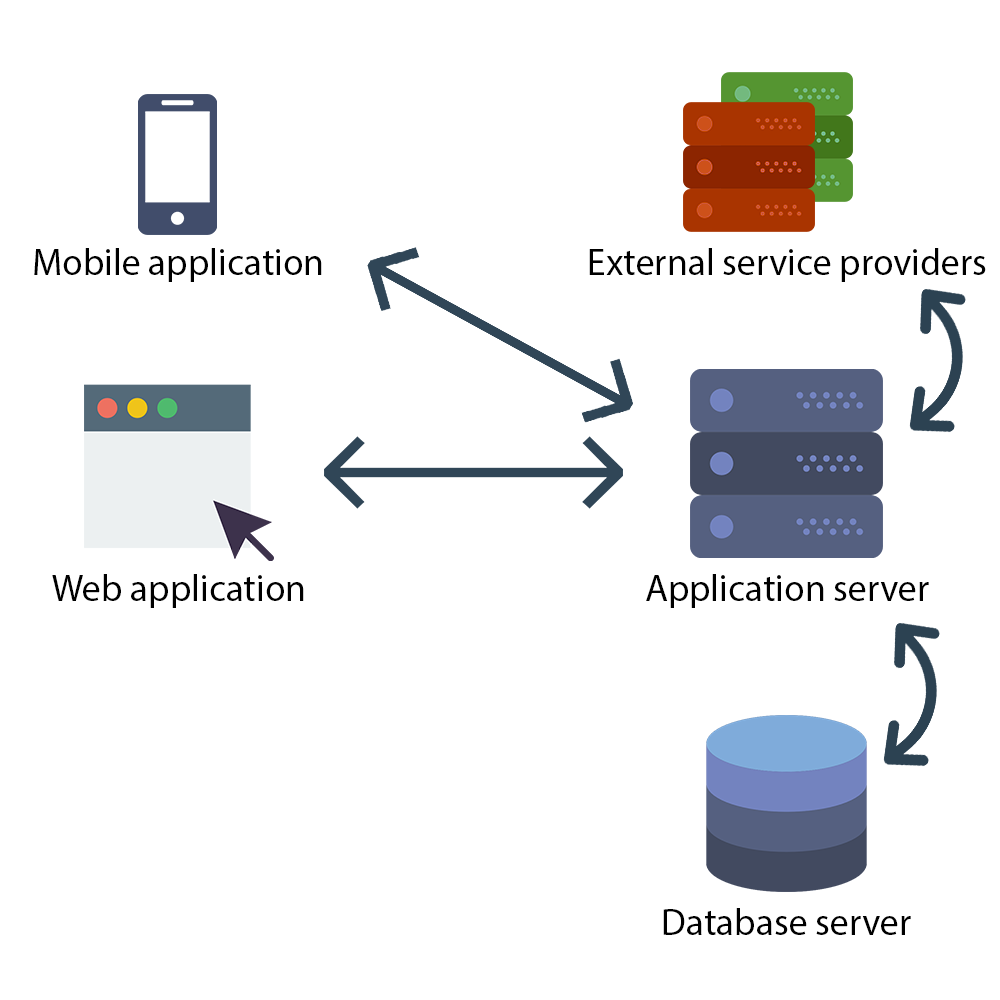
\includegraphics[width=\linewidth]{Images/Architecture/Architecture_design_2.png}
			\caption{Architecture's Ideal Concept}
			\label{fig:AC}
			\end{figure}
			\paragraph{}
Even if Travlendar+ is accessible both with mobile and web browser, it was clear from the beginning that, for this project’s purposes , the application’s strength will lie on the mobile version. Since   
the three‑tier architecture lacks scalability (in fact, it was designed in an era where the idea of elasticity and rapid scaling did not broadly exist) a four-tier one was chosen. Four-tier was recently introduced for mobile applications, so it is the best fit. This way it is also guaranteed that different types of client can share the same application logic. 
			\begin{figure}[H]
			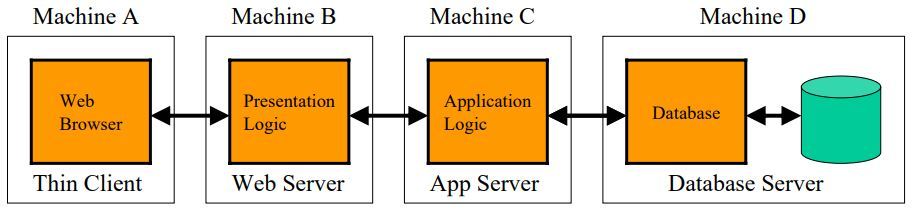
\includegraphics[width=\linewidth]{Images/Architecture/4_Tier_Architecture.jpg}
			\caption{Four Tier Architecture Paradigm Example}
			\label{fig:4TA}
			\end{figure}
			\paragraph{}
The layers are:
			\begin{itemize}
			\item{}\textbf{Client Tier:} Clients’ interfaces and local part of the application.
			\item{}\textbf{Presentation logic Tier:} Web Servers, responsible of “delivery”, the so-called communication between client and application servers. Here is the REST interface. In this tier the different client types are masked to the Application Servers.
			\item{}\textbf{Application logic Tier:} Cluster computing base where the several operations ( in a CRUD interface)  that can be done through Travlendar+ are processed,  data are acquired from the internal database and it is handled the interaction with external providers and secure third-party APIs. Externals provide access to services (e.g.: ticket buying) or data (e.g.: shortest path).
			\item{}\textbf{Data Tier:} The database server stores all the clients’ data (calendar, settings, etc…); information can be divided into users’ data and payment records (this database has extra security).
			\end{itemize}
			\begin{figure}[H]
			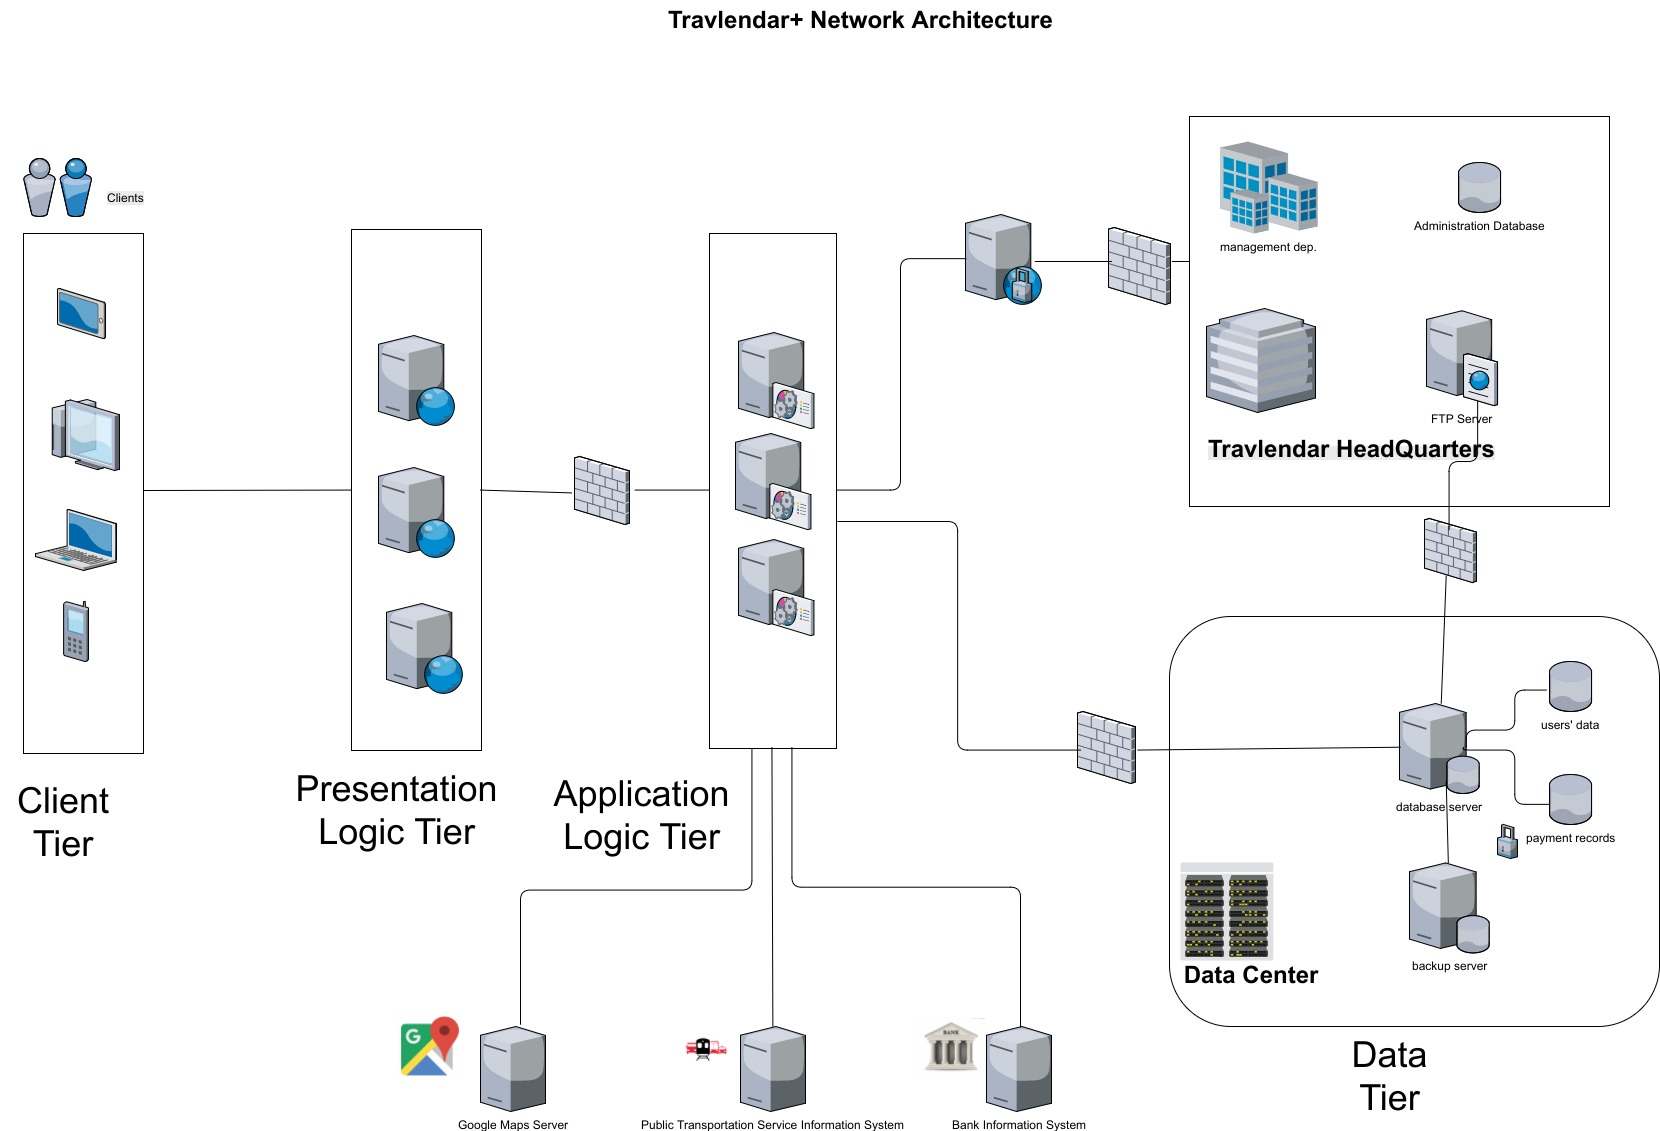
\includegraphics[width=\linewidth]{Images/Architecture/Physical_Architecture.jpg}
			\caption{Physical Architecture}
			\label{fig:PA}
			\end{figure}
				\paragraph{}
The top-right section of the picture above shows how Administrators will interact with the different layers: this part will not be treated in this document (it was never mentioned in RASD) and will be implemented with an ERP software the company is willing to buy from COTS market.
		\subsection{Component View}
			\subsubsection{High Level Component Diagram}
The following diagram shows the most important components of the system and which are the interfaces used to communicate and interact between modules.\\
The client side is made of the User Application Service and Employee Web Service, which are related to their counterparts placed on the server, and will interact with these server parts.\\
The server side is divided into two parts:
				\begin{itemize}
				\item{} User Application Service
				\item{} Employee Web Service
				\end{itemize}
The user web and mobile services are almost identical, so we will discuss only one. The Employee Web Service was not discussed in the RASD and is not relevant for the purpose of the application, so we will not discuss it further.
				\begin{figure}[H]
				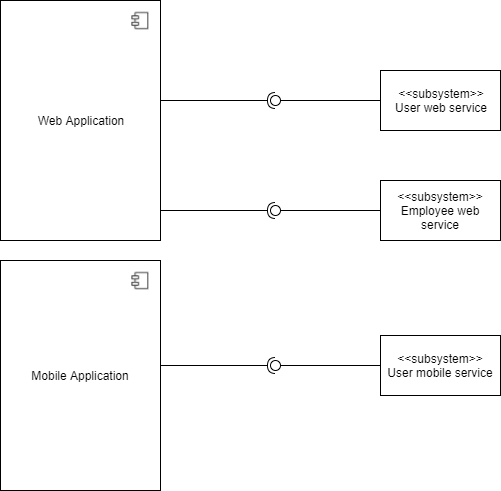
\includegraphics[width=\linewidth]{Images/Architecture/High-Level_Architecture.png}
				\caption{High Level Architecture}
				\label{fig:HLA}
				\end{figure}
			\subsubsection{User Service Application}
This subsystem is composed of five different modules which will provide to the user interfaces to: account management, event management, past events, manage and acquisition of tickets, daily schedule and the vehicle finder.
				\begin{itemize}
				\item{} \textbf{Account Manager:} this module needs to communicate with the DBMS to allow the user to change his account information and preferences.
				\item{} \textbf{Event Module:} this module needs to interact with the maps to retrieve the information of the location of the event and later save it on the database, so it needs to communicate with the DBMS.
				\item{} \textbf{Ticket Module:} this module will have to communicate with three different systems, first of all the tickets bought will have to come directly from the Public Transportation System, so it will need to interact with the PTS. To pay for the ticket it will need to contact a Payment Gateway, and later save the information on the account’s information, so il will need to interact with the DBMS.
				\item{} \textbf{Schedule Module:} this module has to retrieve information about the events and the public transportation schedules from the DB through the DBMS and then calculate the movements through Google Maps API.
				\item{} \textbf{Vehicle Module:} this module simply needs to find the vehicles from their respective systems and show them to the user, which means that will have to interact both with Google Maps and the Vehicle Services.
				\end{itemize}
				\begin{figure}[H]
				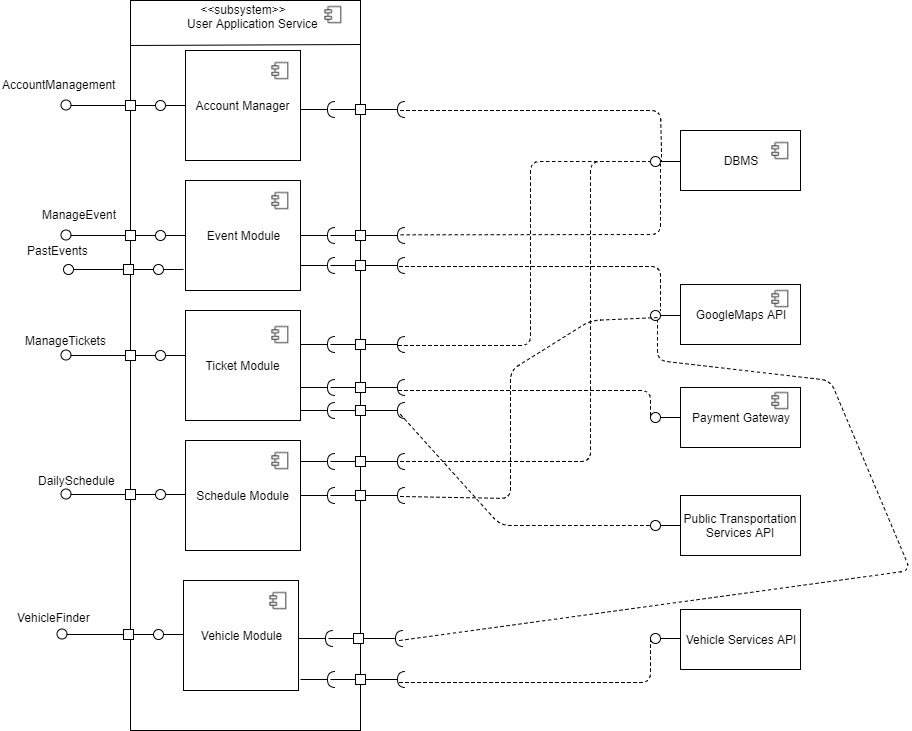
\includegraphics[width=\linewidth]{Images/Architecture/User_Application_Service.png}
				\caption{User Application Service Subsystem}
				\label{fig:UAS}
				\end{figure}
			\newpage
		\subsection{Deployment View}
			\paragraph{}In this section we now match all components (section 2.2) with Travlendar+ hardware architecture (a brief overview was given in section A). If we take a look back to the diagram in Section A, the architecture is compliant with the Java EE model:
			\begin{itemize}
			\item{} Client Presentation Tier $\longleftrightarrow$ Client Tier
			\item{} Web Tier $\longleftrightarrow$ Presentation Logic Tier
			\item{} Business Tier $\longleftrightarrow$ Application Logic Tier
			\item{} Data Tier $\longleftrightarrow$ Data Tier
			\end{itemize}
			\paragraph{}Therefore the application is very likely to be developed in Java and in a JavaEE environment ( NetBeans 8.2 or Eclipse Oxygen)
			\paragraph{}Since Travlendar+ aims to reach the highest number of users, the system must handle a future high load of connections. For this purpose there is going to be more than one Apache HTTP  server in the web tier and a cluster base in business tier. This multiplicity of machines will need load balancers  to exploit their computational power in handling connections and executing parallel tasks in application layer. Data are stored in an external and independent Relational Database (MS SQL server), as shown in section 2.1. 
				\begin{figure}[H]
				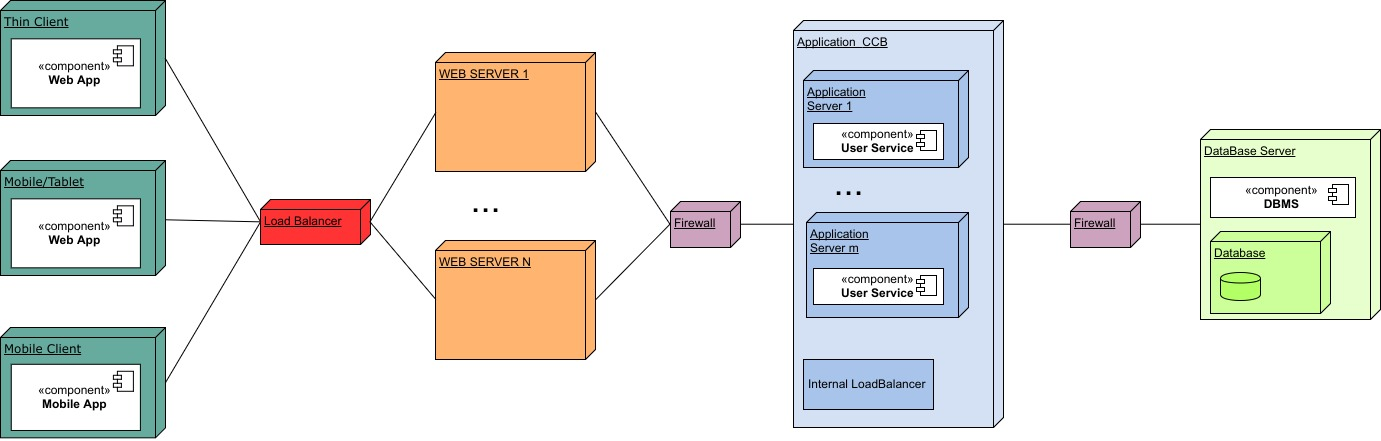
\includegraphics[width=\linewidth]{Images/Architecture/Deployment3.jpg}
				\caption{Deployment}
				\label{fig:D}
				\end{figure}
			\paragraph{}The web and application servers will be implemented starting from open source Java EE Apache Servers’ code. Moreover, to allow a safer client-server communication, HTTPS encryption will be enabled on web servers. Interaction between Business and Data tier will be through a ODBC.
		\subsection{Runtime View}
			\paragraph{}In this section all Sequence Diagrams previously showed in the RASD will be proposed in more details. In the previous document,  Travlendar+’s system was modeled as one entity (one lifeline in sequence diagrams); now it will be decomposed in the main subsystems and modules. The following diagrams are to give a high level snapshot of various components’ interactions, in cases of interest.  
				\subsubsection{Create Account}
				\begin{figure}[H]
				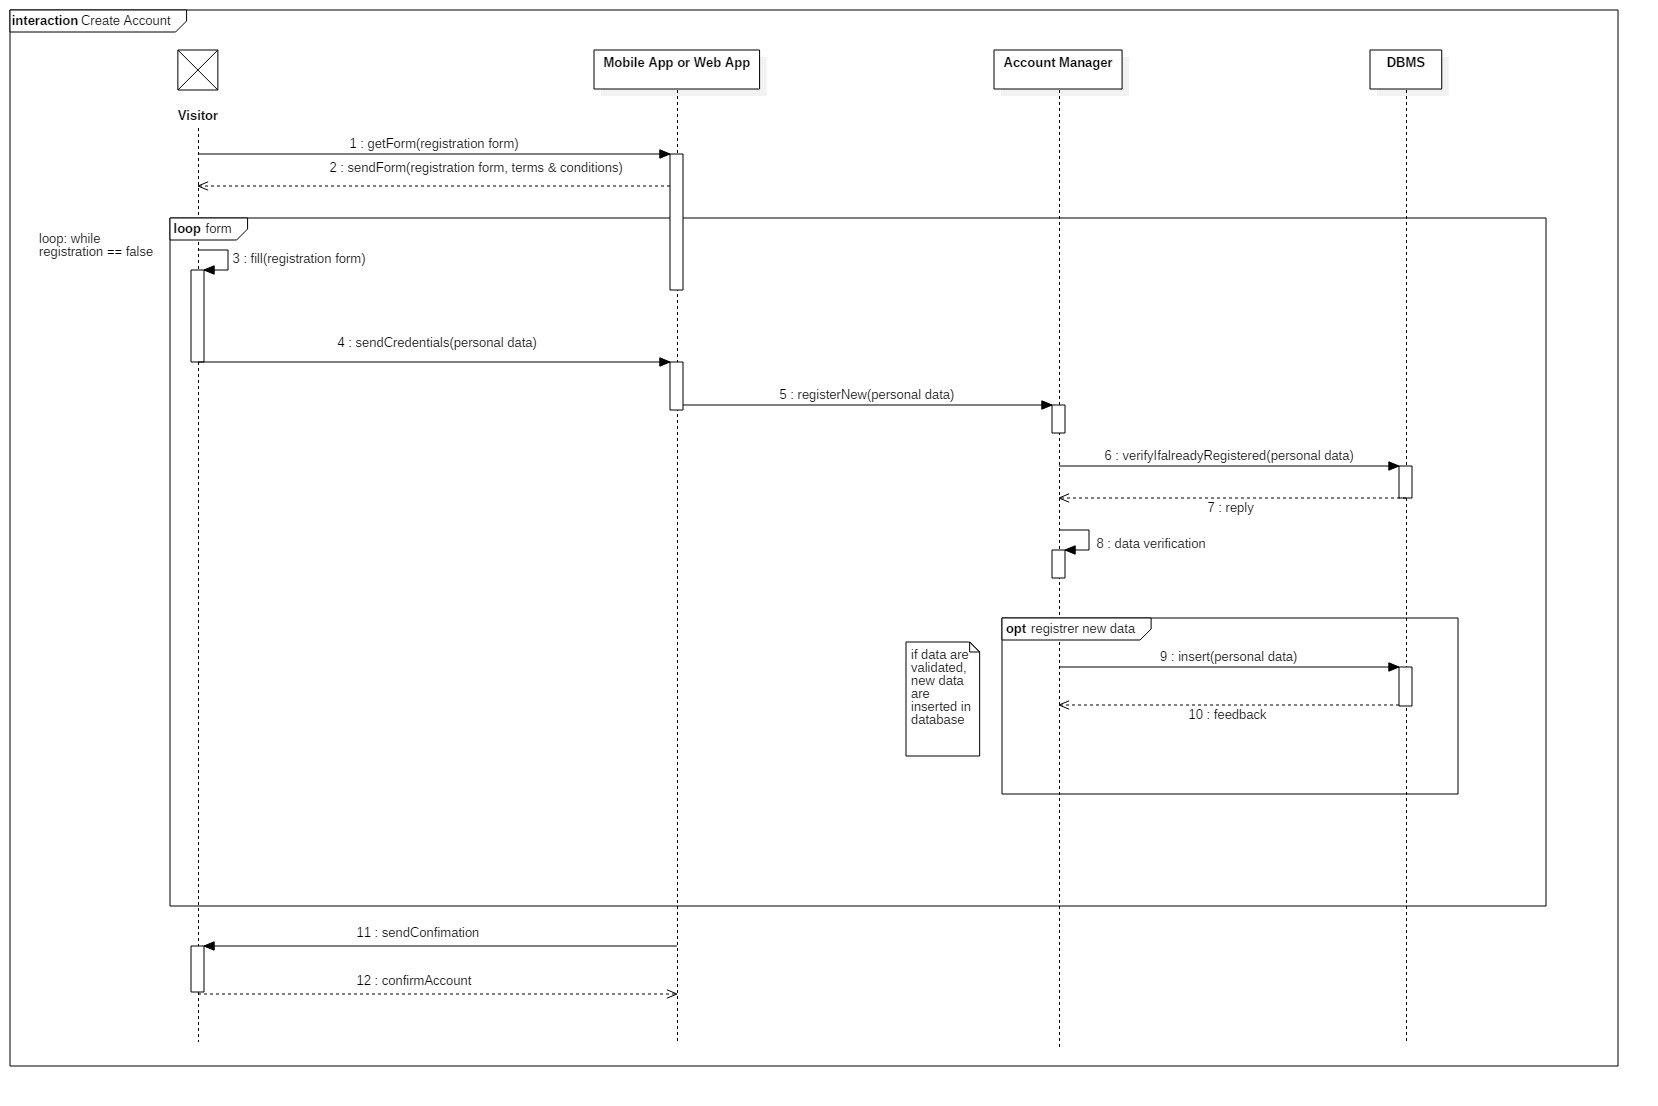
\includegraphics[width=\linewidth]{Images/Sequence_Diagrams/1-Create_Account_DD.jpg}
				\caption{Create Account}
				\label{fig:SD1}
				\end{figure}
				\subsubsection{Login}
				\begin{figure}[H]
				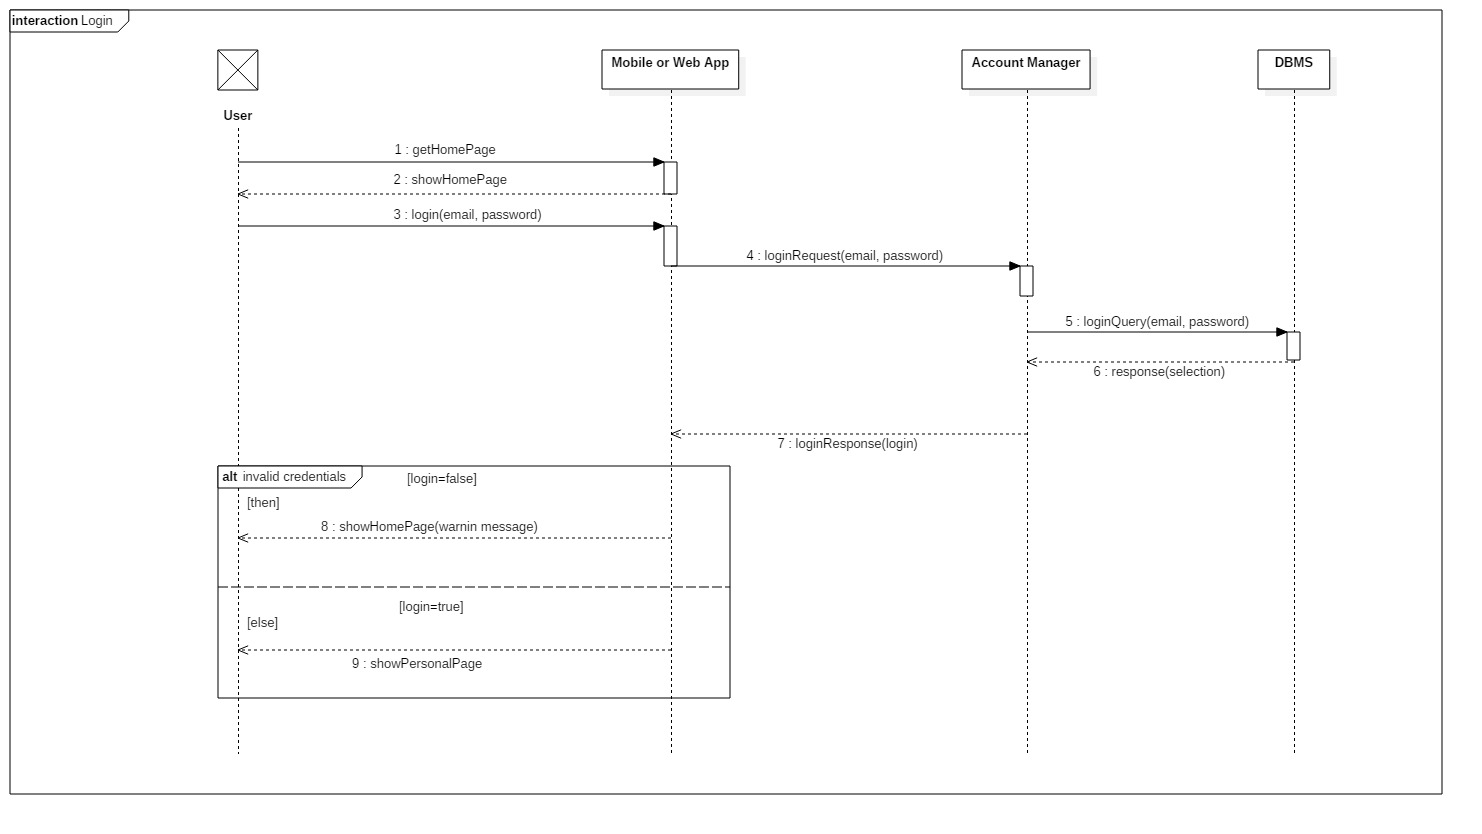
\includegraphics[width=\linewidth]{Images/Sequence_Diagrams/2-Login_DD.jpg}
				\caption{Login}
				\label{fig:SD2}
				\end{figure}
				\subsubsection{Create Event}
				\begin{figure}[H]
				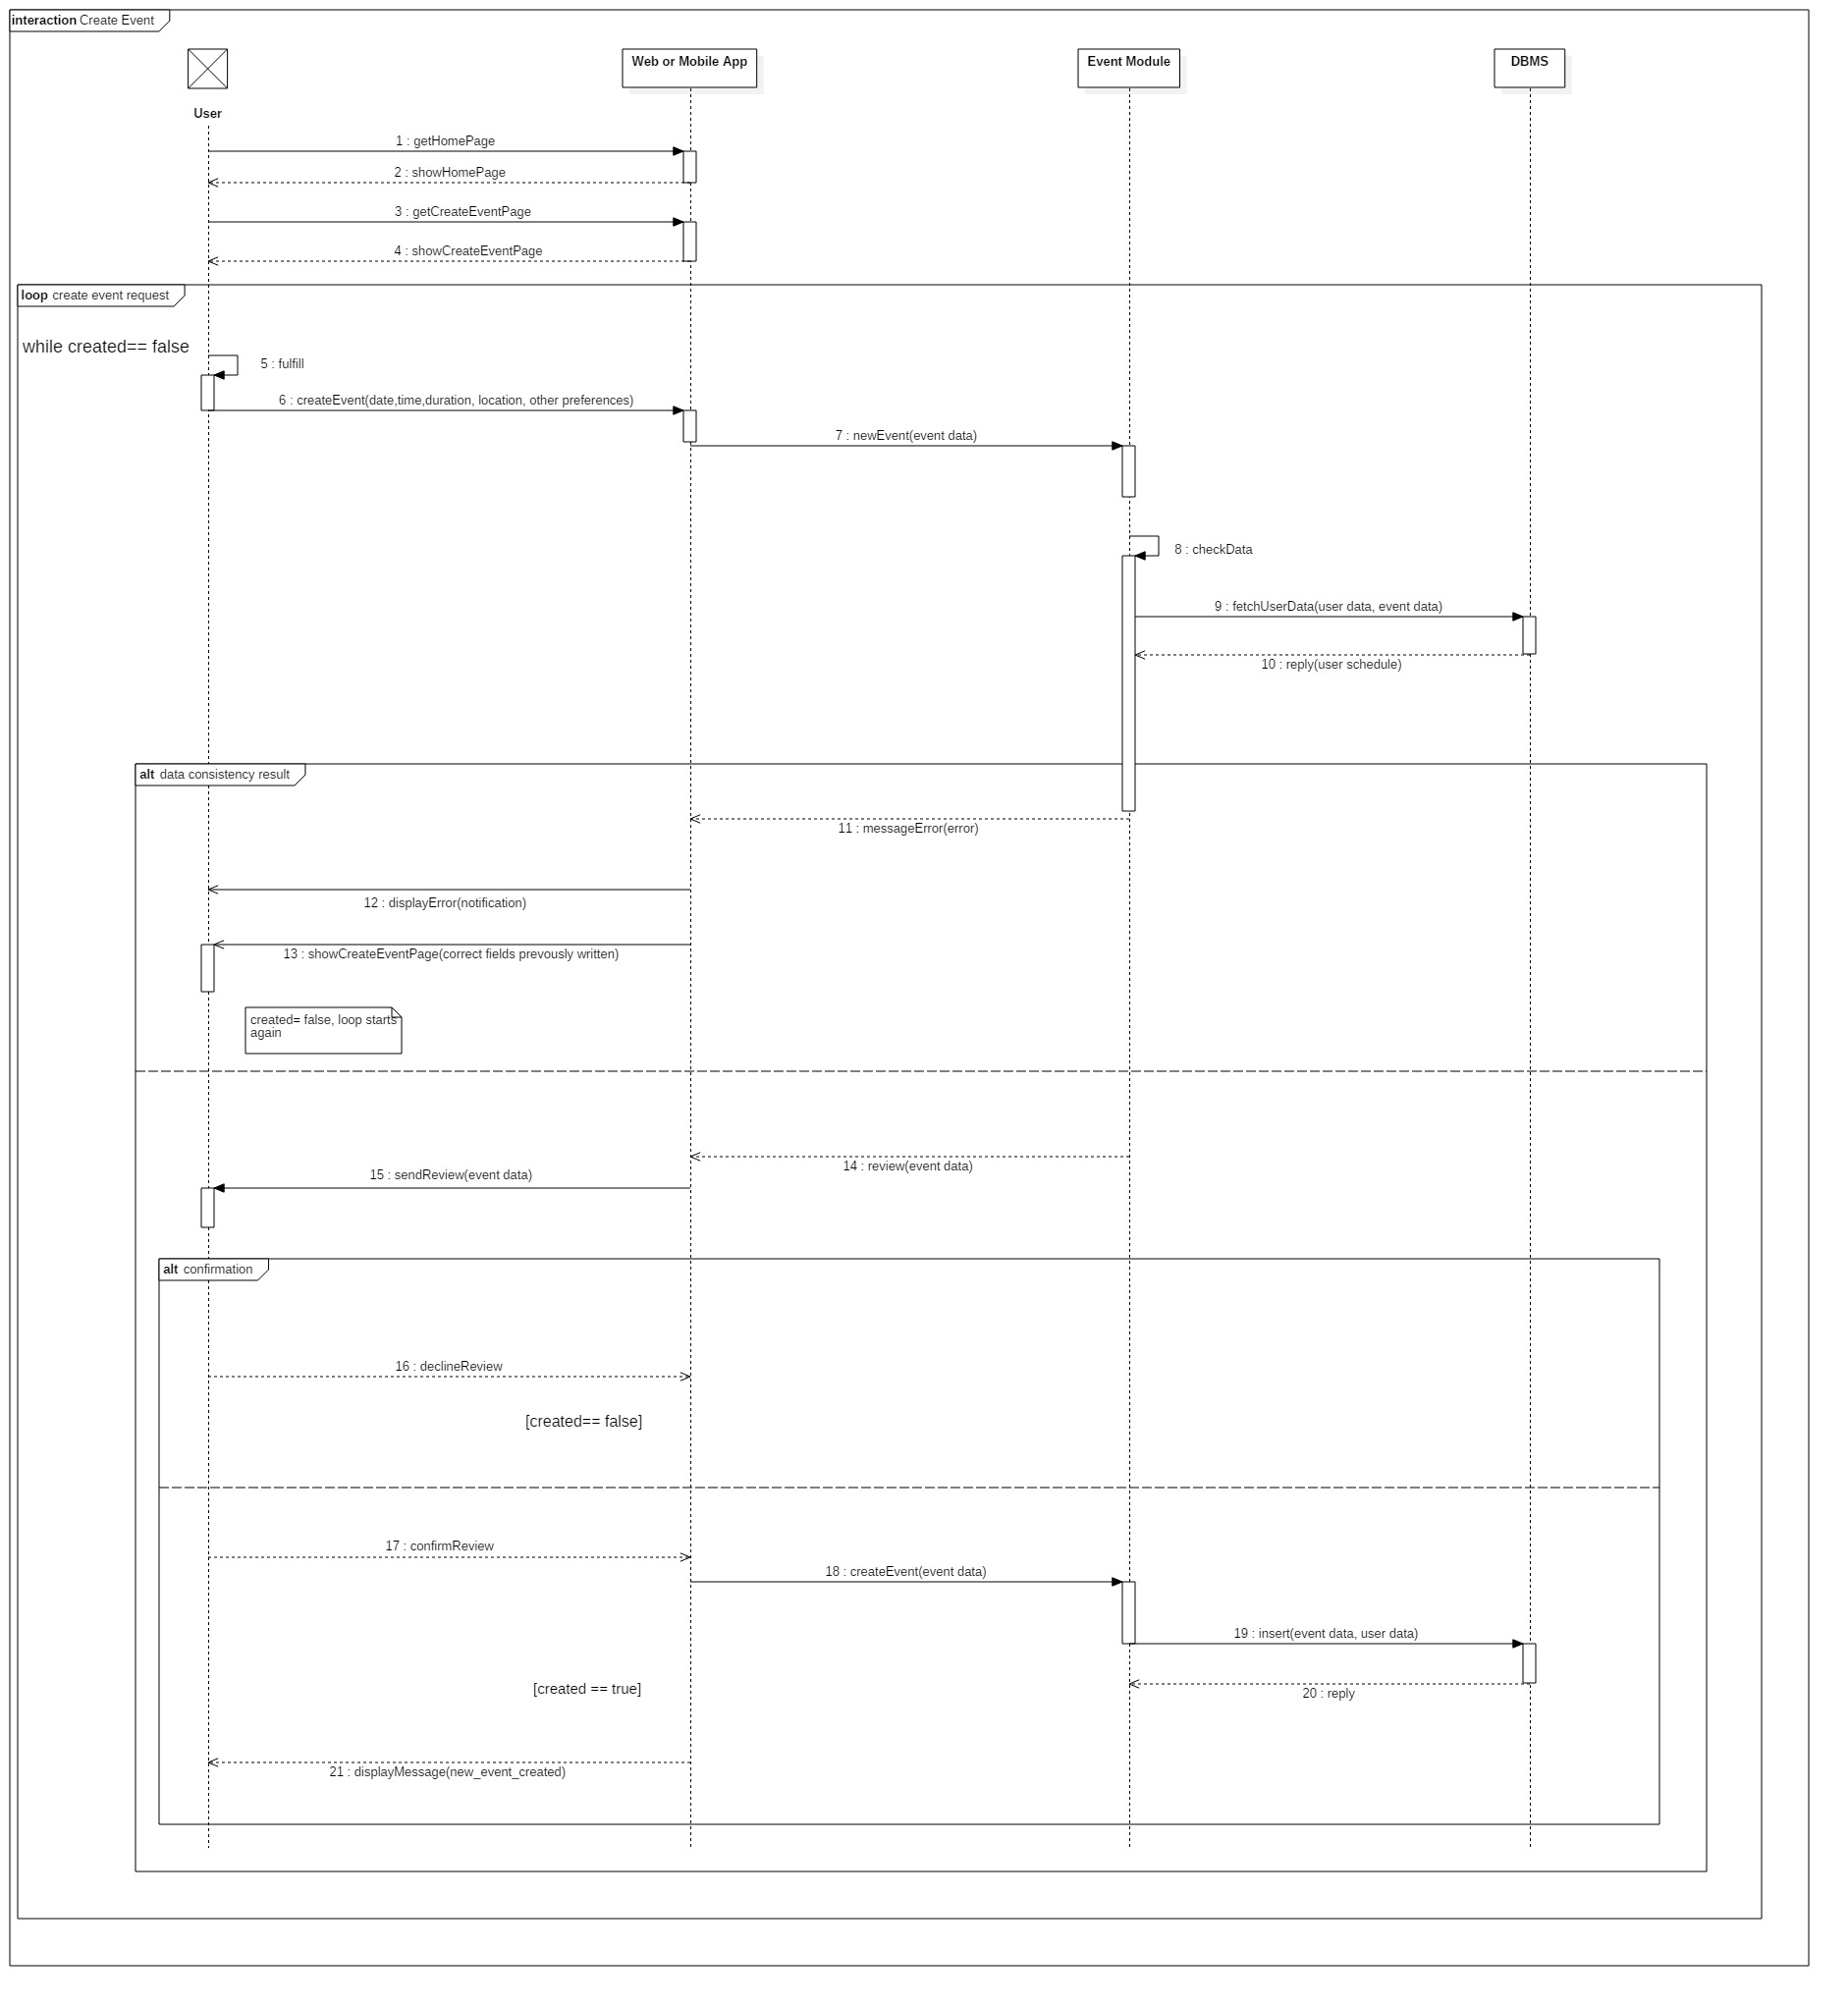
\includegraphics[width=\linewidth]{Images/Sequence_Diagrams/3-Create_Event_DD.jpg}
				\caption{Create Event}
				\label{fig:SD3}
				\end{figure}
				\subsubsection{Accept Path}
				\begin{figure}[H]
				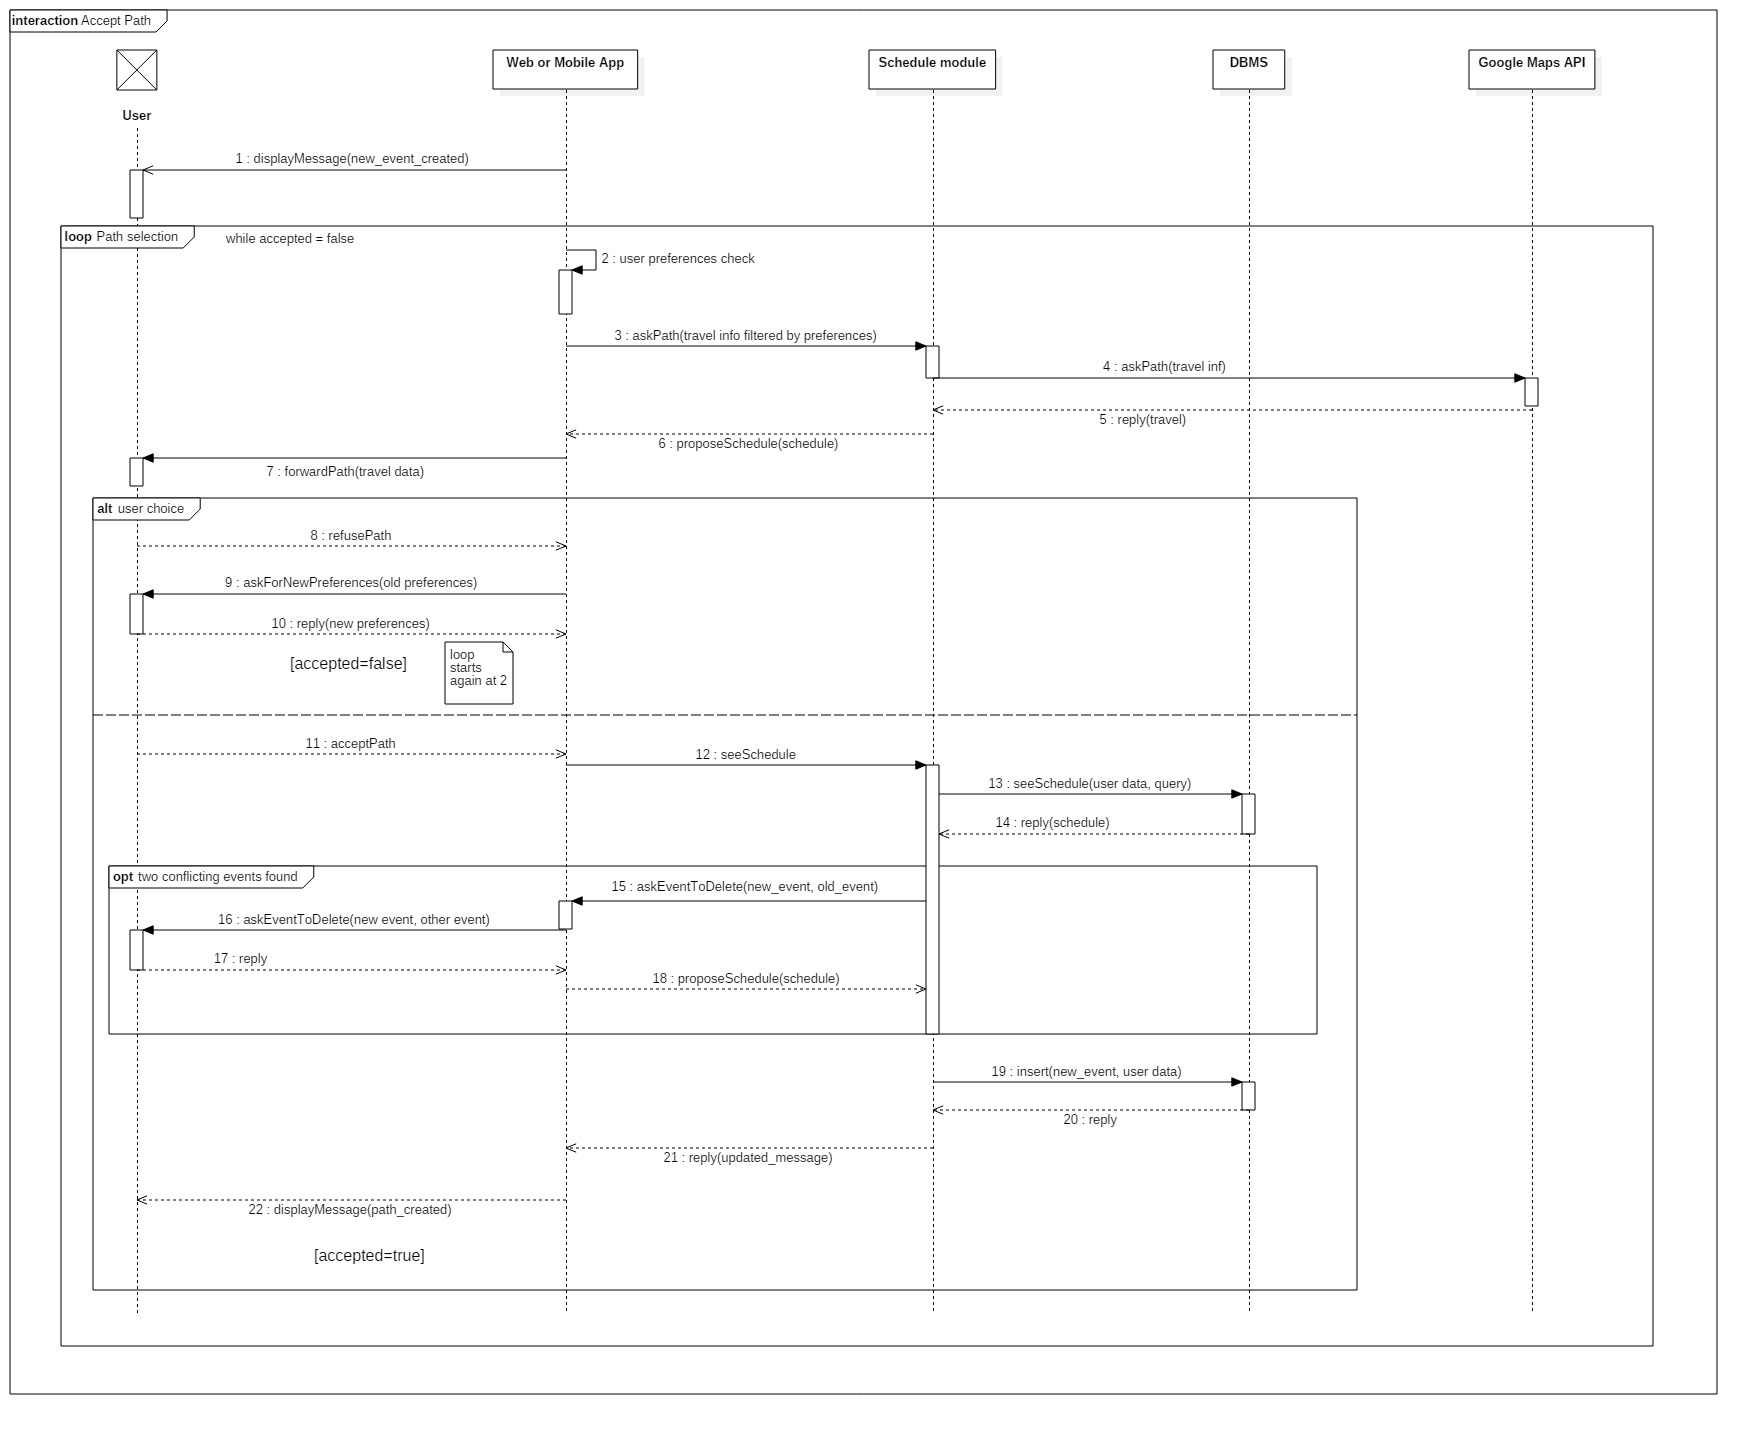
\includegraphics[width=\linewidth]{Images/Sequence_Diagrams/4-Accept_Path_DD.jpg}
				\caption{Accept Path}
				\label{fig:SD4}
				\end{figure}
				\subsubsection{Buy Ticket}
				\begin{figure}[H]
				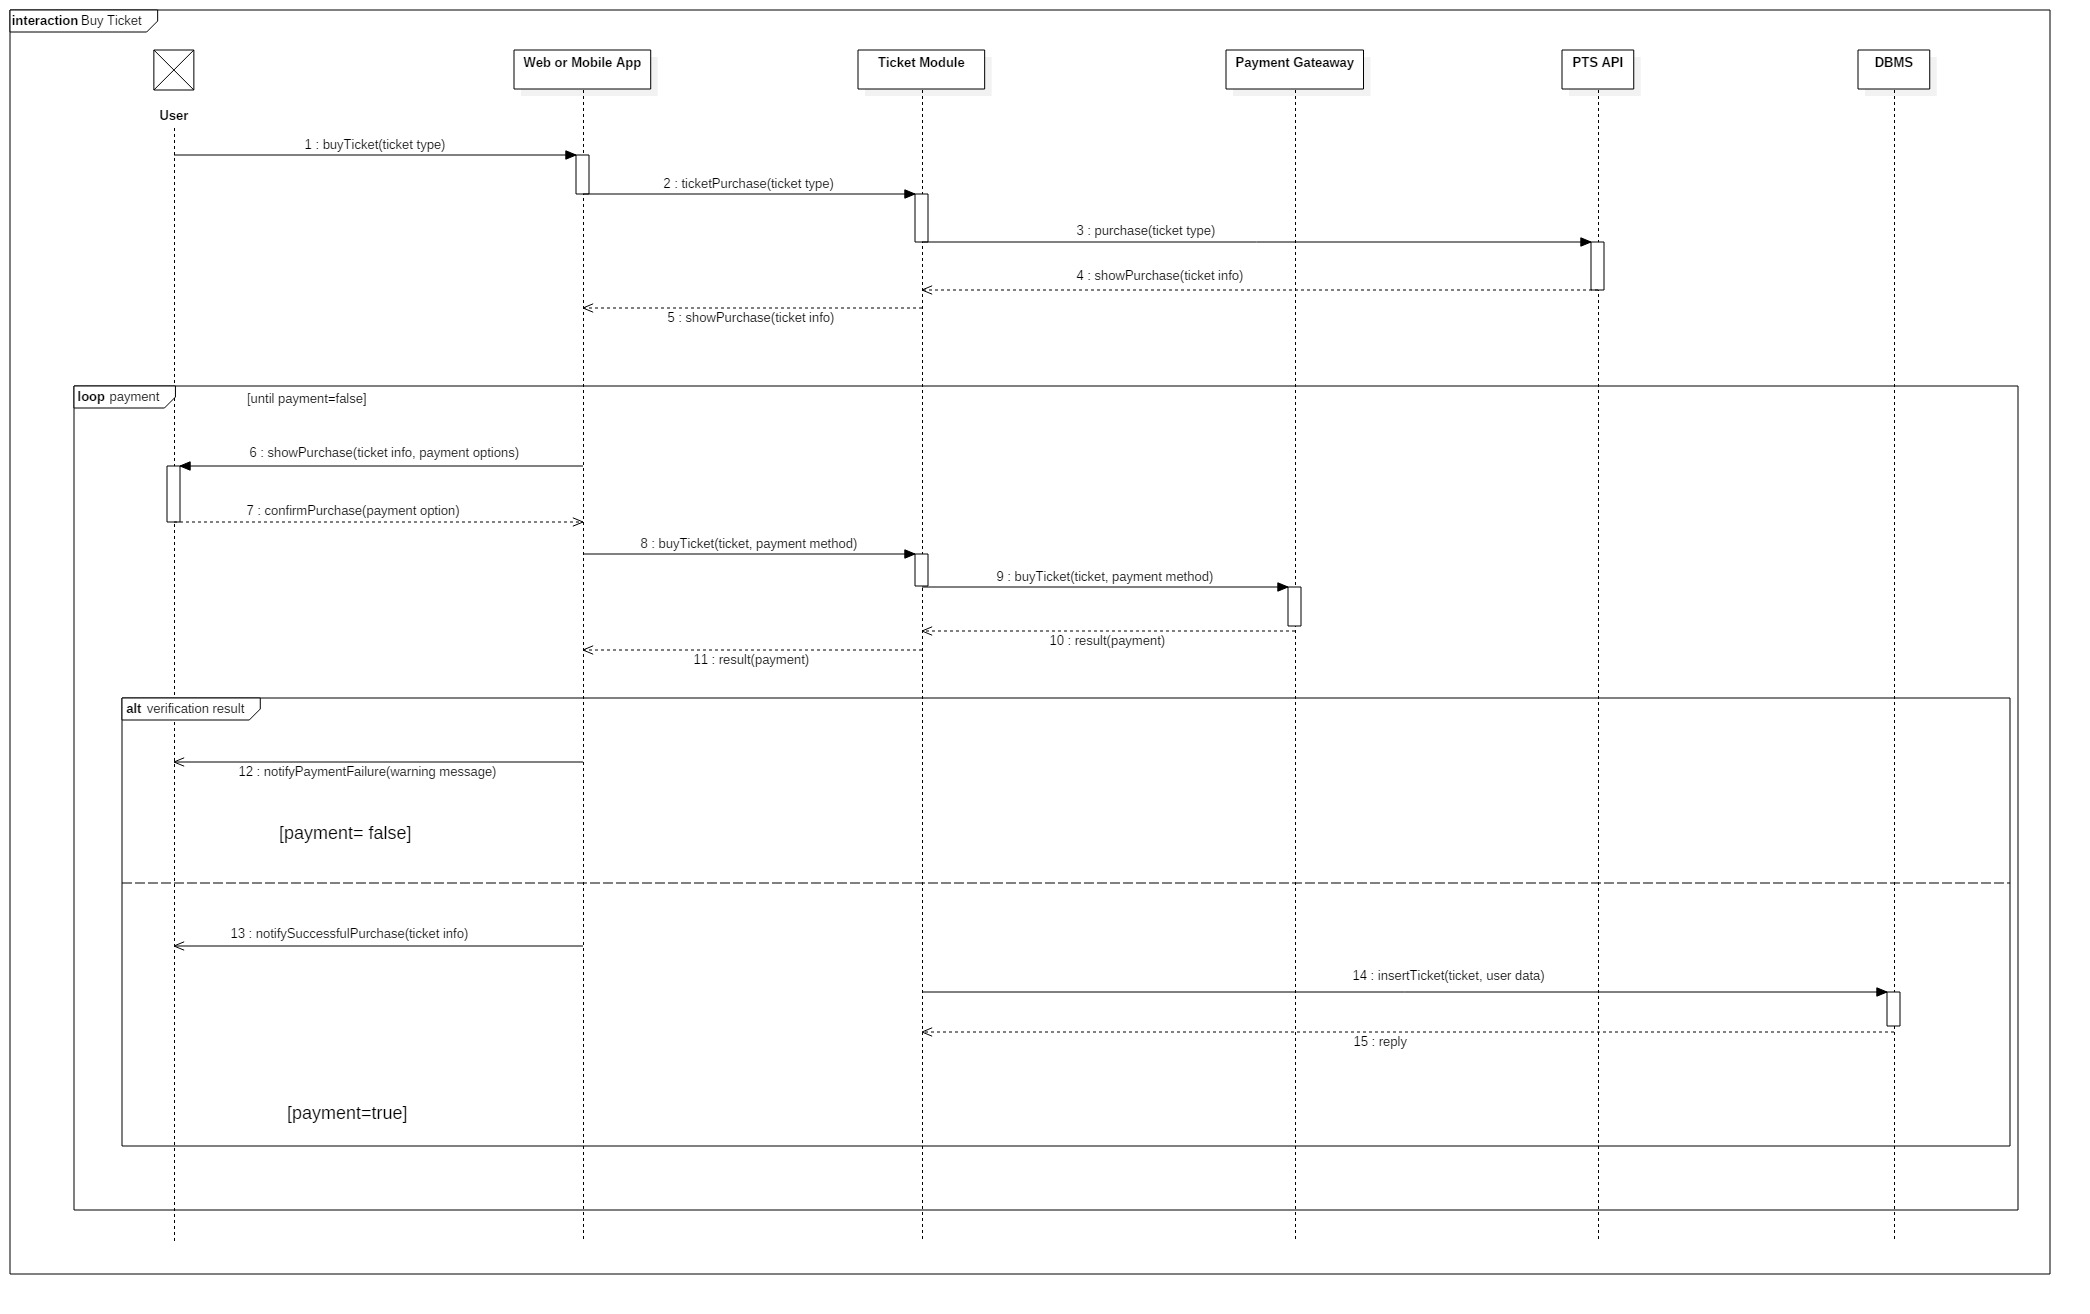
\includegraphics[width=\linewidth]{Images/Sequence_Diagrams/5-Buy_Ticket_DD.jpg}
				\caption{Buy Ticket}
				\label{fig:SD5}
				\end{figure}
				\subsubsection{Activate Ticket}
				\begin{figure}[H]
				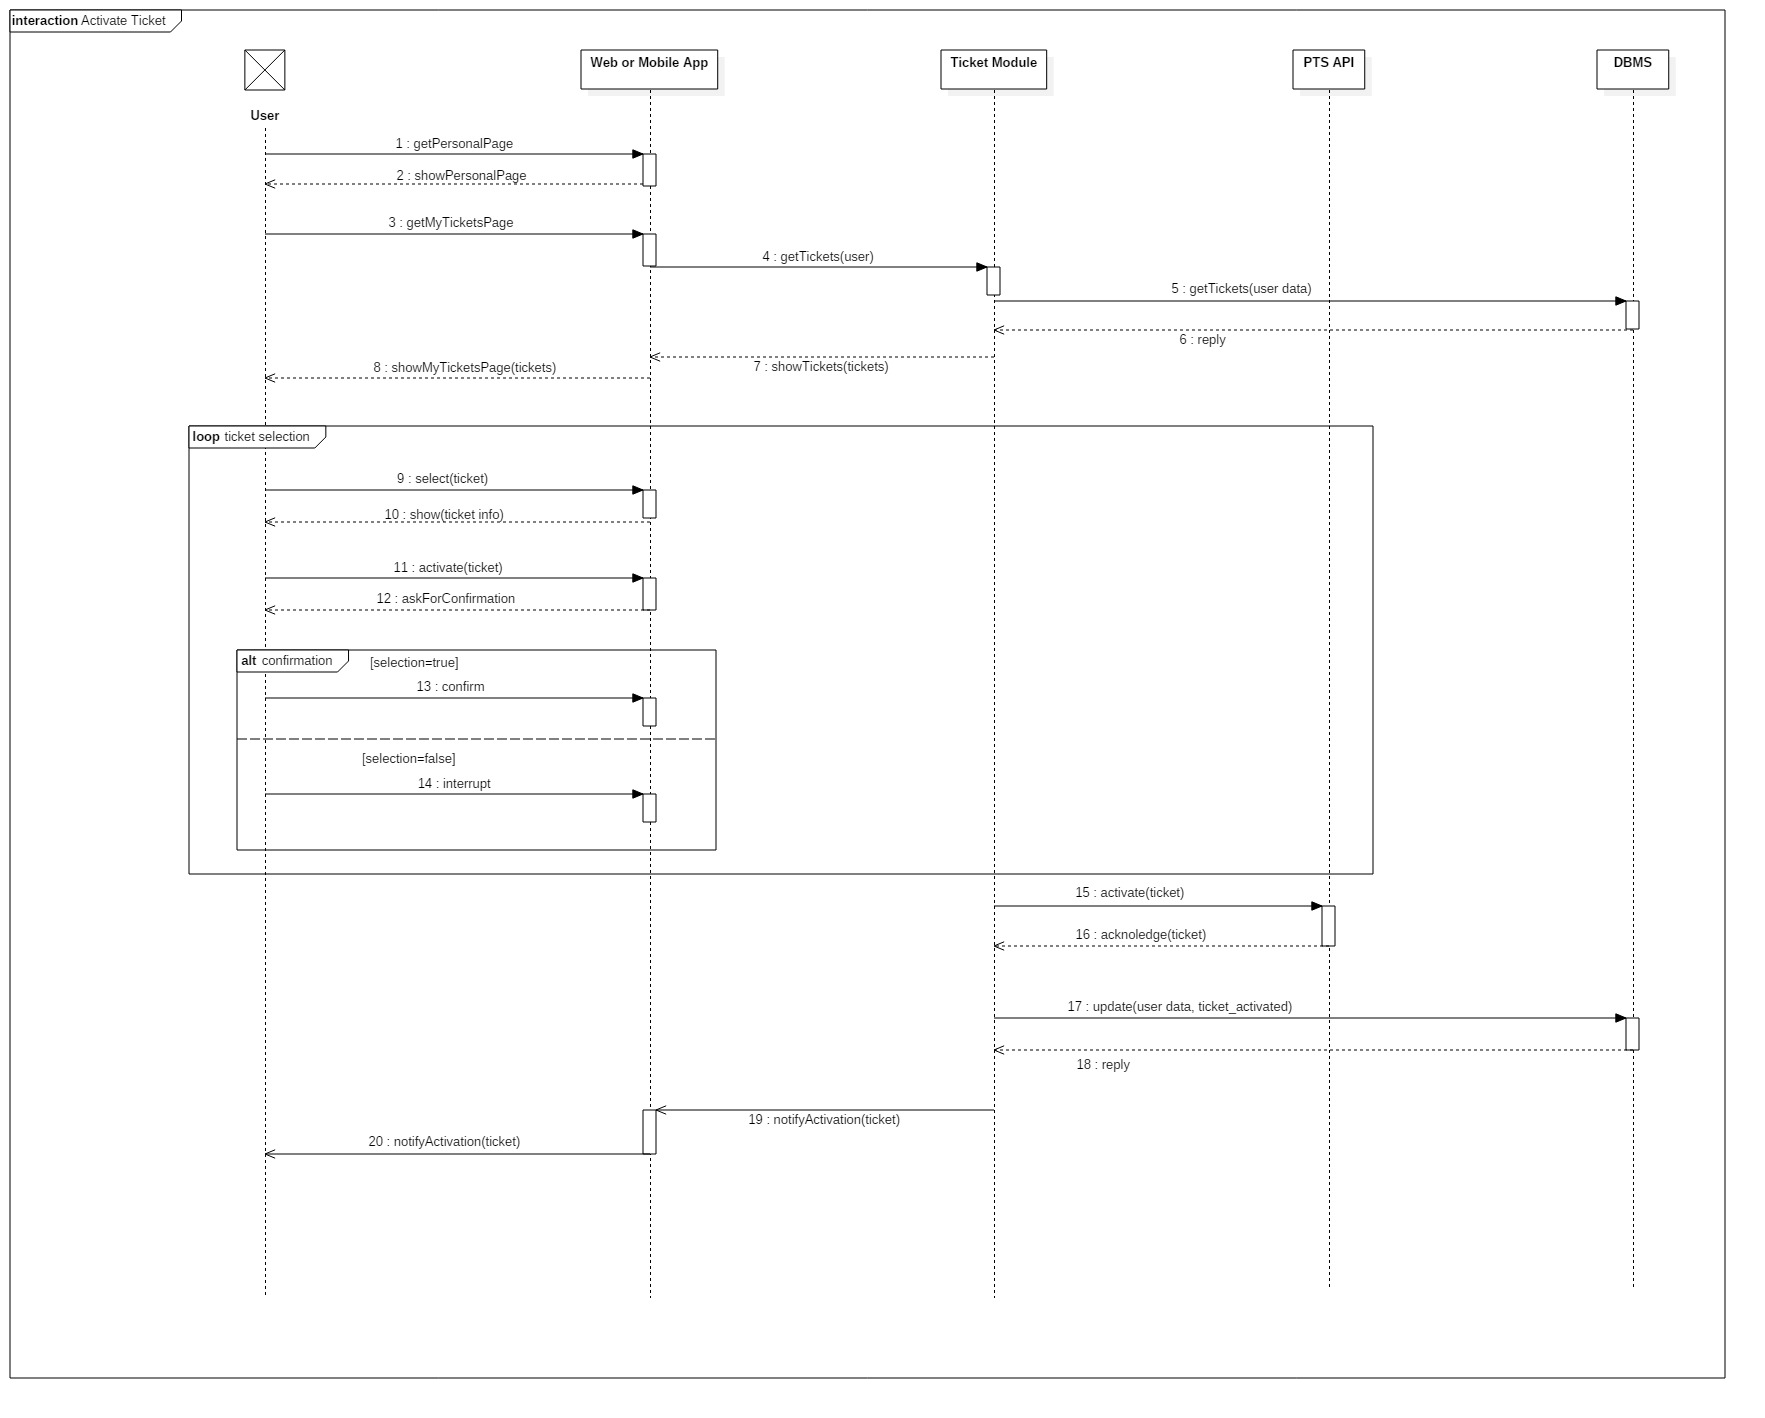
\includegraphics[width=\linewidth]{Images/Sequence_Diagrams/6-Activate_Ticket_DD.jpg}
				\caption{Activate Ticket}
				\label{fig:SD6}
				\end{figure}
				\subsubsection{Find Vehicle}
				\begin{figure}[H]
				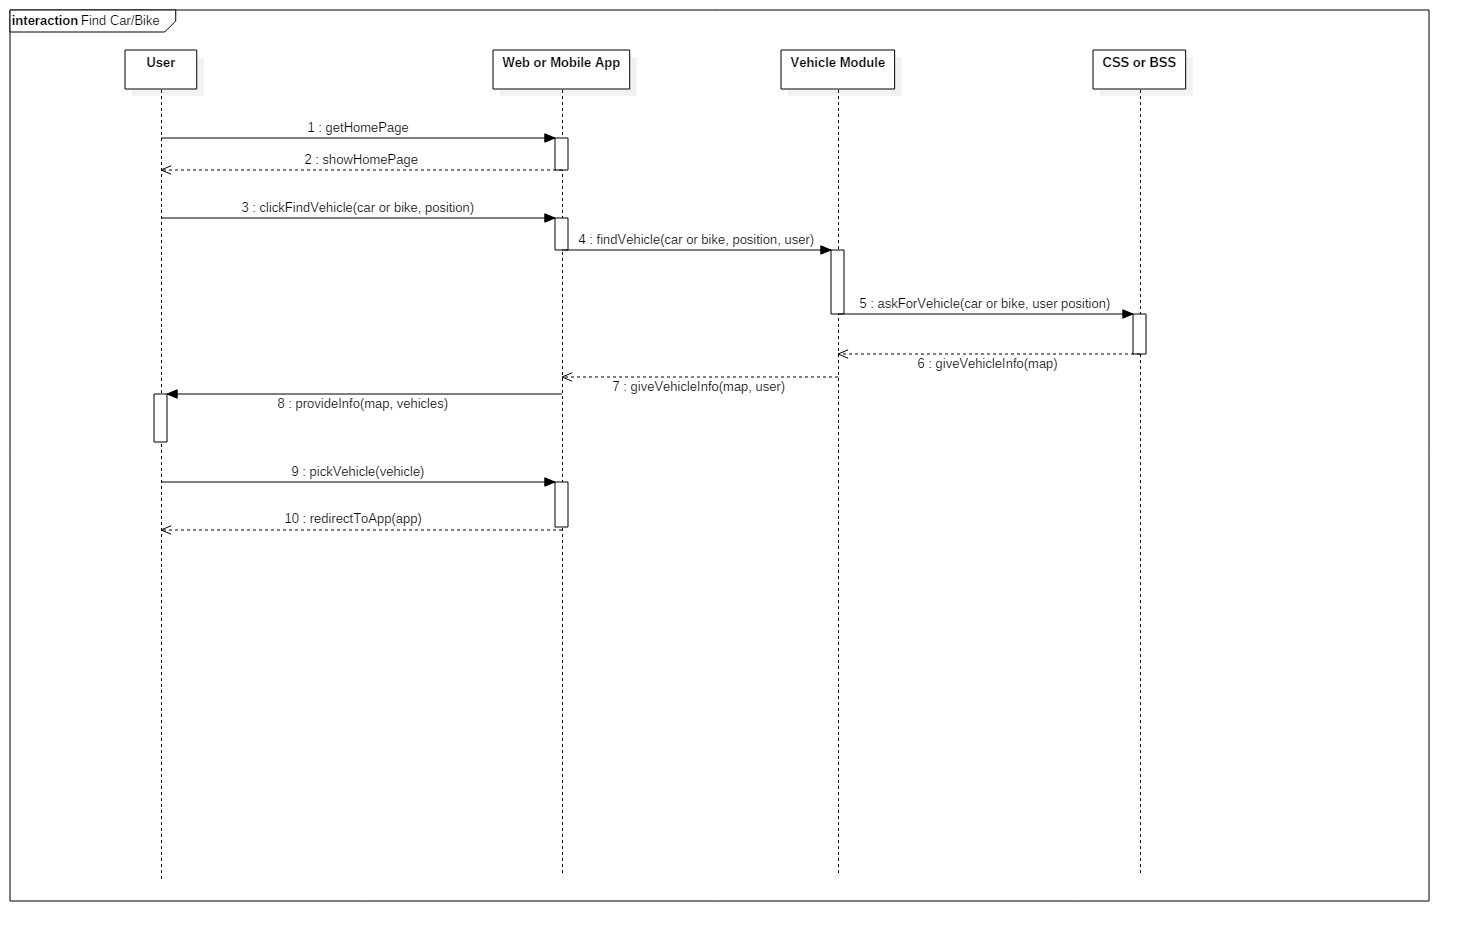
\includegraphics[width=\linewidth]{Images/Sequence_Diagrams/7-Find_Car_Bike_DD.jpg}
				\caption{Find Vehicle}
				\label{fig:SD7}
				\end{figure}
				\subsubsection{Load Balance}
				\begin{figure}[H]
				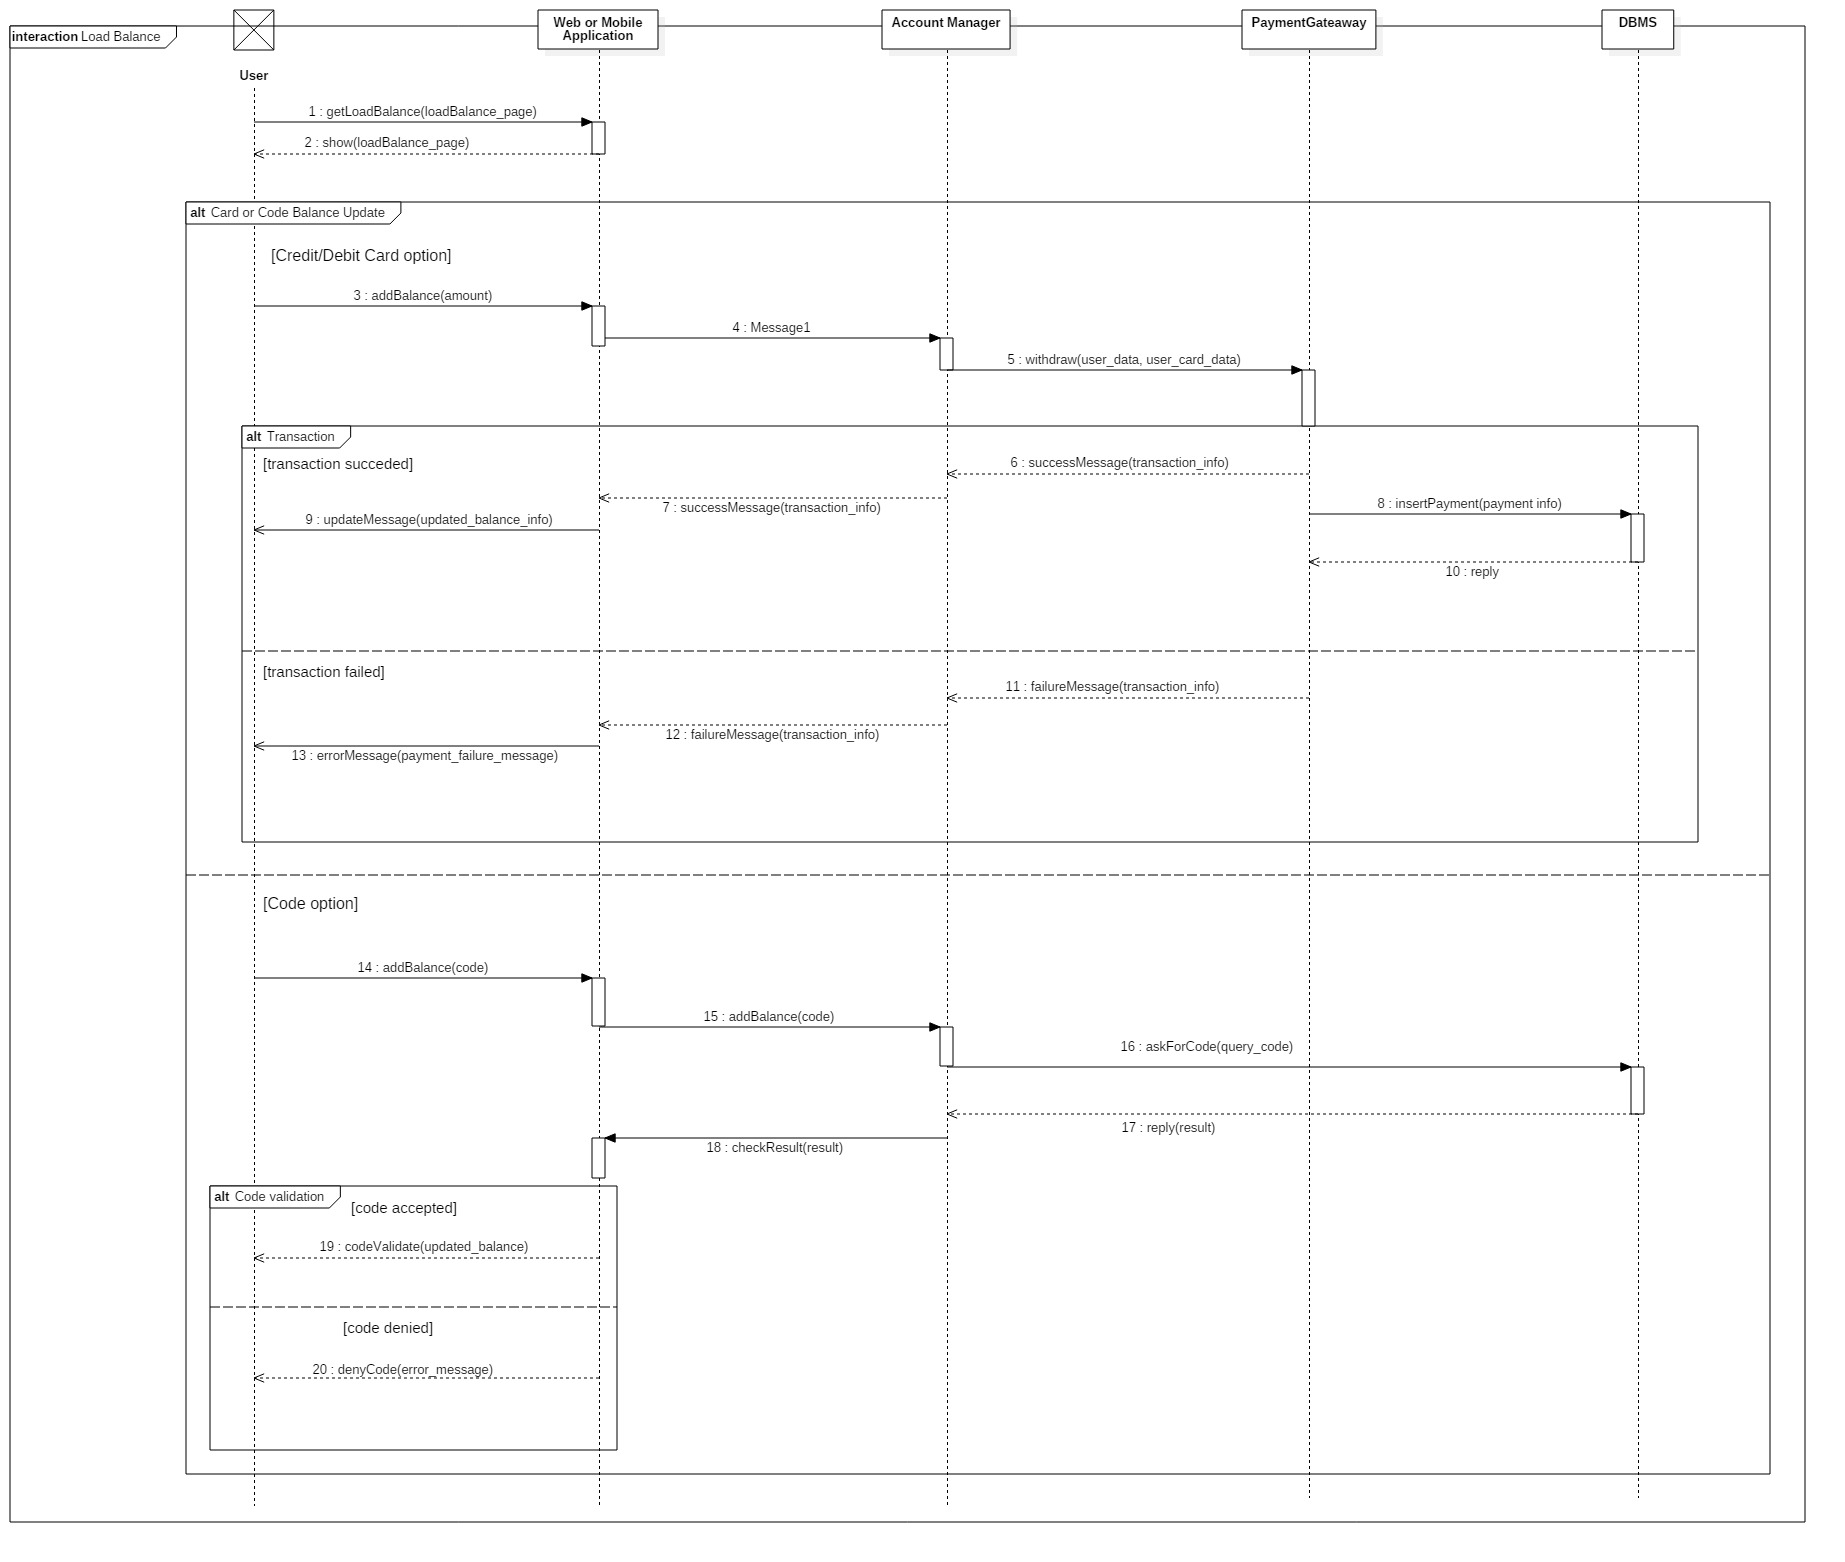
\includegraphics[width=\linewidth]{Images/Sequence_Diagrams/8-Load_Balance_DD.jpg}
				\caption{Load Balance}
				\label{fig:SD8}
				\end{figure}
		\subsection{Component Interfaces}
			\paragraph{} The diagram below shows the main methods that belong to the User Application Server. This subsystem is composed of five modules, which, through their methods, provide the client with the functionalities that the users need to use Travlendar+, such as creating an account, creating an event, buying tickets, etc.
				\begin{figure}[H]
				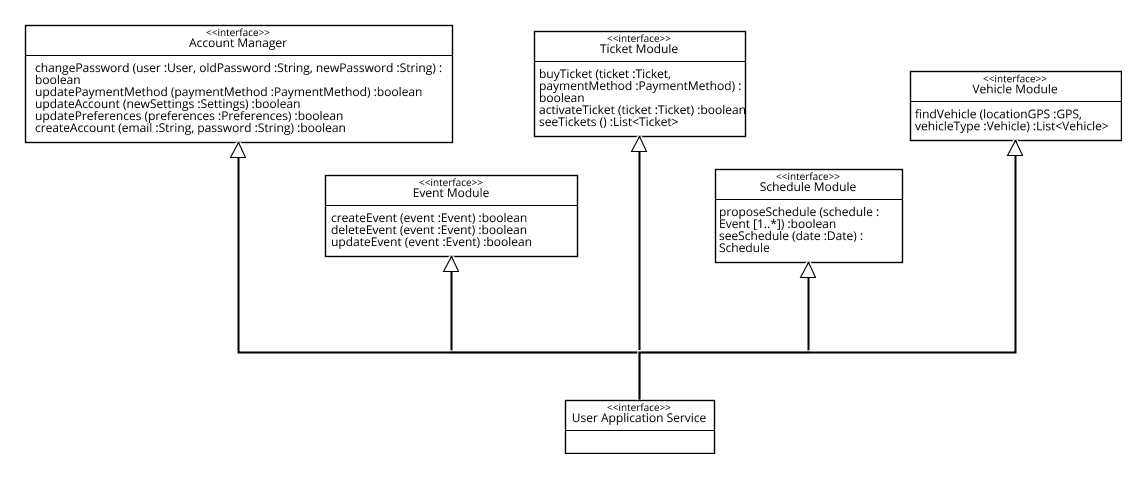
\includegraphics[width=\linewidth]{Images/Architecture/Interface_Methods.png}
				\caption{Component Interfaces}
				\label{fig:CI	}
				\end{figure}
		\subsection{Selected Architectural Styles and Patterns}
			\paragraph{} The following patterns are recommended for the implementation of the project:
				\begin{itemize}
				\item{} \textbf{Model-View-Controller: } this pattern divides the software into three different components, dividing how the information is shown to the user from how it is represented in the system.
				\item{} \textbf{Proxy Pattern: }through this pattern we can use an object as an interface for another object.
				\item{} \textbf{Factory Pattern: }this pattern allows to create objects leaving the process of creation to subclasses.
				\item{} \textbf{Visitor Pattern: }this pattern is really useful to change the executing algorithm of a class, depending on which class is visiting the object.
				\item{} \textbf{Observer Pattern: }it is necessary to implement the MVC Pattern.
				\item{} \textbf{State Pattern: }this pattern allows a class to change its behaviour based on its current state.
				\end{itemize}
			\paragraph{} During the implementation we will update this list citing any pattern that we will use and are not in the paragraph above.
		\newpage
		\subsection{Other Design Decisions}
			\paragraph{Maps APIs\\}
Since the app needs to track the position of our users during the day we need to render maps on the operating systems that will support Travlendar+. To be able to do this we will use Google Maps API to track the user’s position.
			\paragraph{Weather Tracking\\}
The application has to keep track of the weather conditions to decide which are the suggested vehicles, which means that we will have to connect the application to an external weather system in order to give the correct information to the user and the application.
		\newpage
	\section{Algorithm Design}
		\paragraph{}The main task of Travlendar+ is to notify the user of any problem or reminder in his daily schedule. The computation of distances and paths is committed to an external navigation system, which returns only the results. In the following Java-like pseudocode, this external system is referenced as “navigationService”.
		\subsection{Notifications}
			\paragraph{}The server keeps a list of candidate notifications with a future timestamp. Every minute, the server looks for the notifications with a timestamp equal to the current time and checks other variables to determine if the notification must be delivered (e.g.: if an event occurs within the same time it takes to move to its location and the user has not left yet, the conditions are met to send a “late” notification).\\ 
			\begin{figure}[H]
			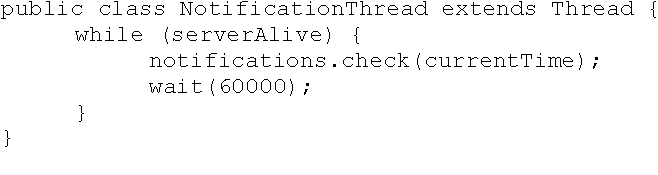
\includegraphics[width=0.8\linewidth]{Algorithm_PDFs/NotificationThread-cropped.pdf}
			\caption{}
			\label{fig:C1}
			\end{figure}
		\subsection{External Navigation System}
			\paragraph{}The server interacts with an external actor who provides paths computation. This actor is referenced by the server as an object.
			\begin{figure}[H]
			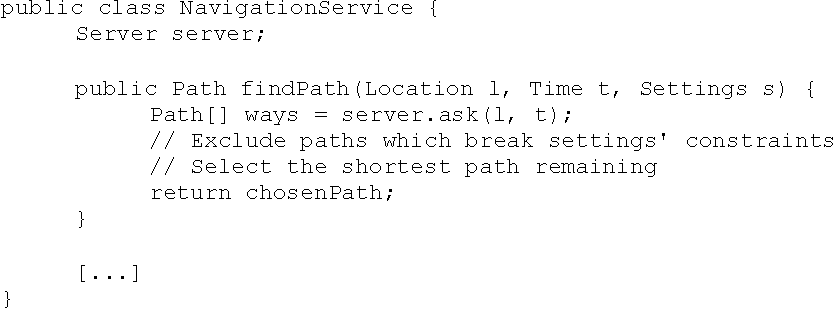
\includegraphics[width=0.8\linewidth]{Algorithm_PDFs/NavigationService-cropped.pdf}
			\caption{}
			\label{fig:C2}
			\end{figure}
			\paragraph{\\} The object’s method findPath returns a Path.
			\begin{figure}[H]
			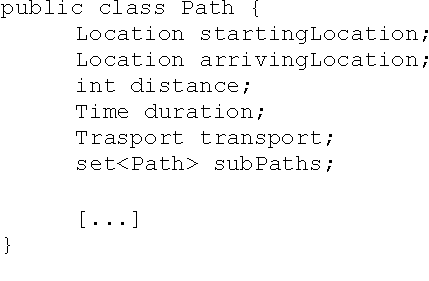
\includegraphics[width=0.5\linewidth]{Algorithm_PDFs/Path-cropped.pdf}
			\caption{}
			\label{fig:C3}
			\end{figure}
		\subsection{Event Creation}
			\paragraph{}Creating an event involves interacting with the external navigation system and adding a new notification to the system.\\
			\begin{figure}[H]
			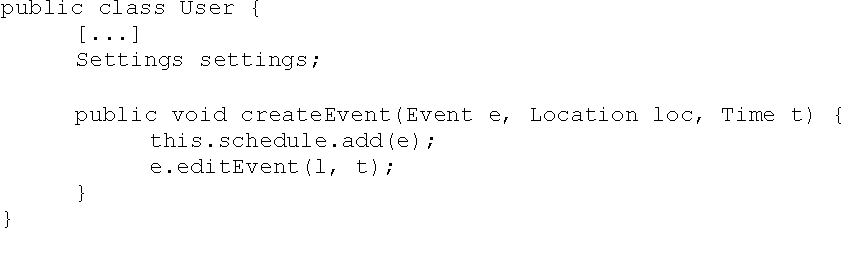
\includegraphics[width=0.8\linewidth]{Algorithm_PDFs/User-cropped.pdf}
			\caption{}
			\label{fig:C4}
			\end{figure}
			\begin{figure}[H]
			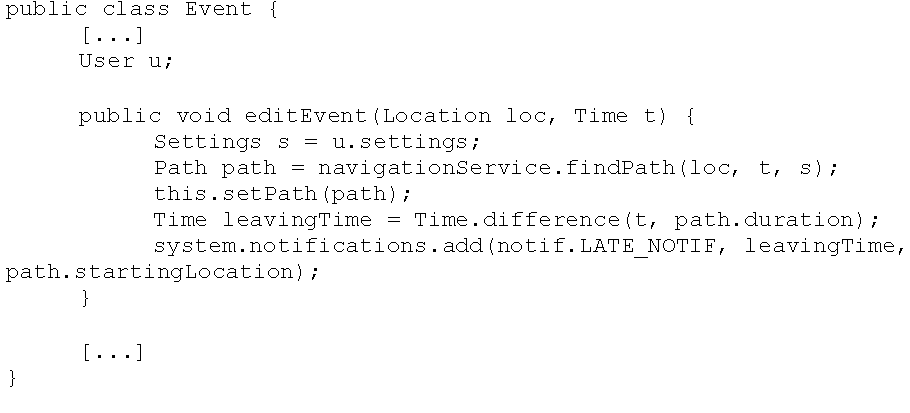
\includegraphics[width=0.8\linewidth]{Algorithm_PDFs/Event-cropped.pdf}
			\caption{}
			\label{fig:C5}
			\end{figure}
		\subsection{User Settings}
			\paragraph{}The system keeps reference to the user’s settings in the user’s object. The settings contain a set of contraints and a method to check them all with given transport and time.\\
			\begin{figure}[H]
			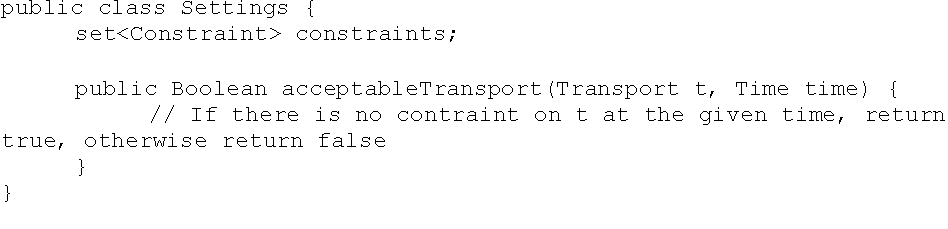
\includegraphics[width=0.8\linewidth]{Algorithm_PDFs/Settings-cropped.pdf}
			\caption{}
			\label{fig:C6}
			\end{figure}
			\paragraph{}The several types of constraint (lunch, time and transport, transport…) extend an abstrat class overriding the public method “check”.
			\begin{figure}[H]
			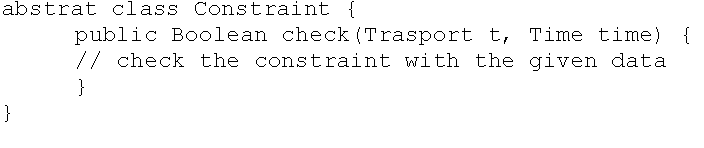
\includegraphics[width=0.8\linewidth]{Algorithm_PDFs/Constraint-cropped.pdf}
			\caption{}
			\label{fig:C7}
			\end{figure}
		\newpage			
	\section{User Interface Design}
		\paragraph{}Travlendar+ is mainly designed to be used through mobile application, to encourage its usage in movement. Nevertheless, it is also accessible through web application. There is no exclusive operation which can be done only on one of the two appliances.
		\subsection{Mockups}
		\subsubsection{Mobile}
		\paragraph{}On the first access, it will be requested to the user to login or register to the system. If he is creating a new account, the user must also accept the Travlendar+ terms and conditions.\\
			\begin{figure}[H]
			\minipage{0.4\textwidth}
			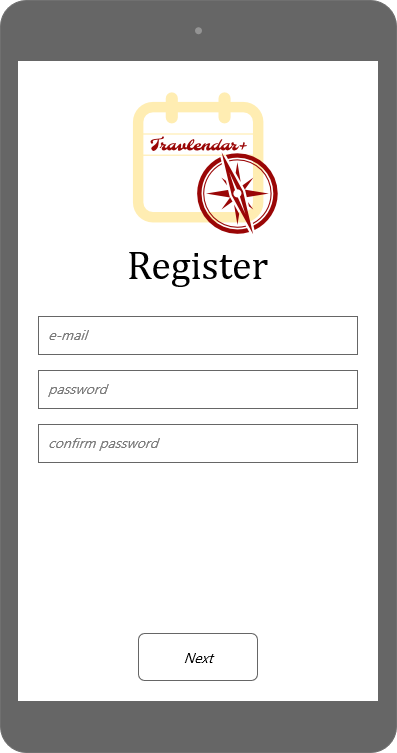
\includegraphics[width=\linewidth]{Images/Mockup/Mobile/01-email_and_password.png}
			\caption{\textbf{Mobile app:} Account Creation}\label{fig:MU1}
			\endminipage\hfill
			\minipage{0.4\textwidth}
			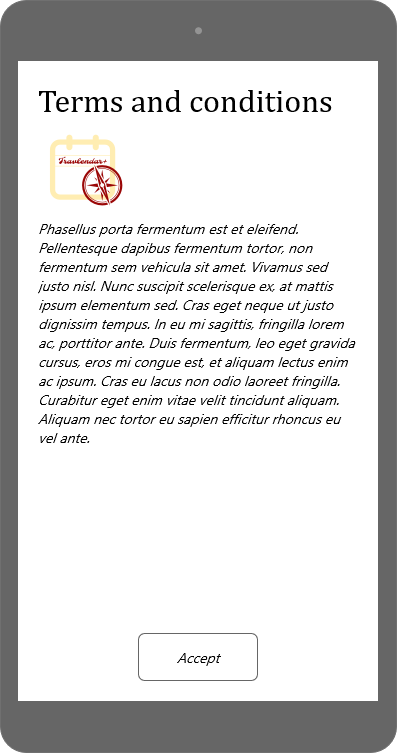
\includegraphics[width=\linewidth]{Images/Mockup/Mobile/02-Terms_and_conditions.png}
  			\caption{\textbf{Mobile app:} Terms and Conditions}\label{fig:MU2}
			\endminipage
			\end{figure}
		\newpage
		\paragraph{}Once the user logins, he accesses the home page and can create a new event.
			\begin{figure}[H]
			\minipage{0.32\textwidth}
			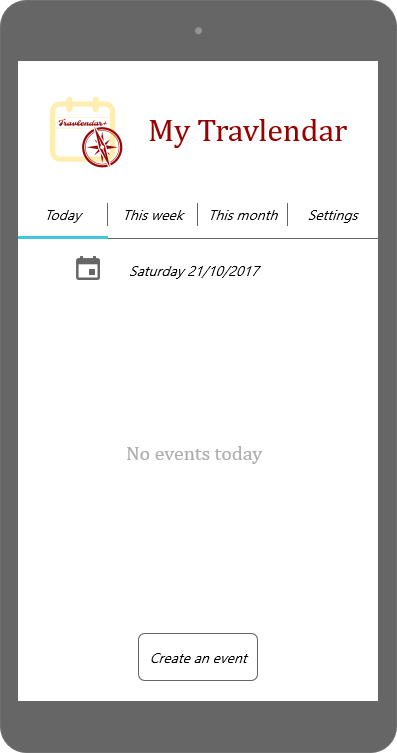
\includegraphics[width=\linewidth]{Images/Mockup/Mobile/03-Home_Page.png}
			\caption{\textbf{Mobile app:} Home Page}\label{fig:MU3}
			\endminipage\hfill
			\minipage{0.32\textwidth}
			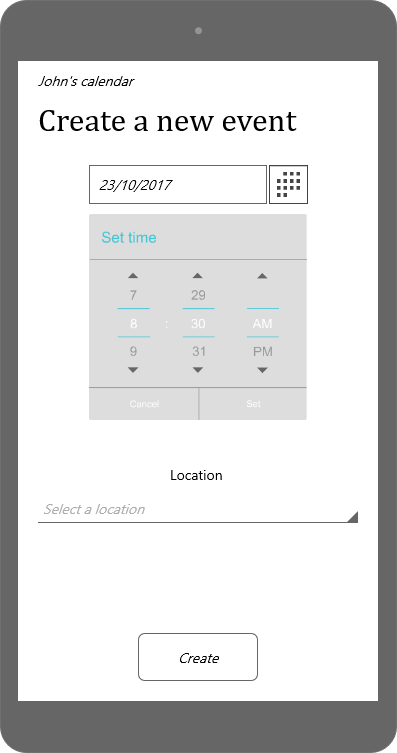
\includegraphics[width=\linewidth]{Images/Mockup/Mobile/04-Create_an_event.png}
  			\caption{\textbf{Mobile app:} Event Creation}\label{fig:MU4}
			\endminipage \hfill
			\minipage{0.32\textwidth}
			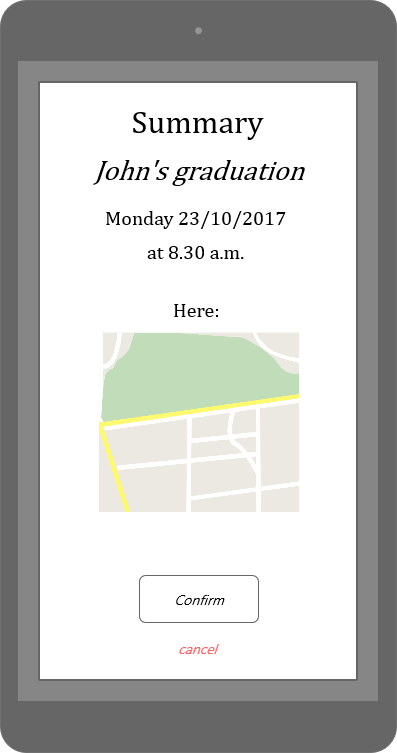
\includegraphics[width=\linewidth]{Images/Mockup/Mobile/05-Summary.png}
			\caption{\textbf{Mobile app:} Event Summary}\label{fig:MU5}
			\endminipage
			\end{figure}
		\newpage
		\subsubsection{Web}
		\paragraph{}The following mockups will show the user interface when using Travlendar+ from a web browser.
			\begin{figure}[H]
			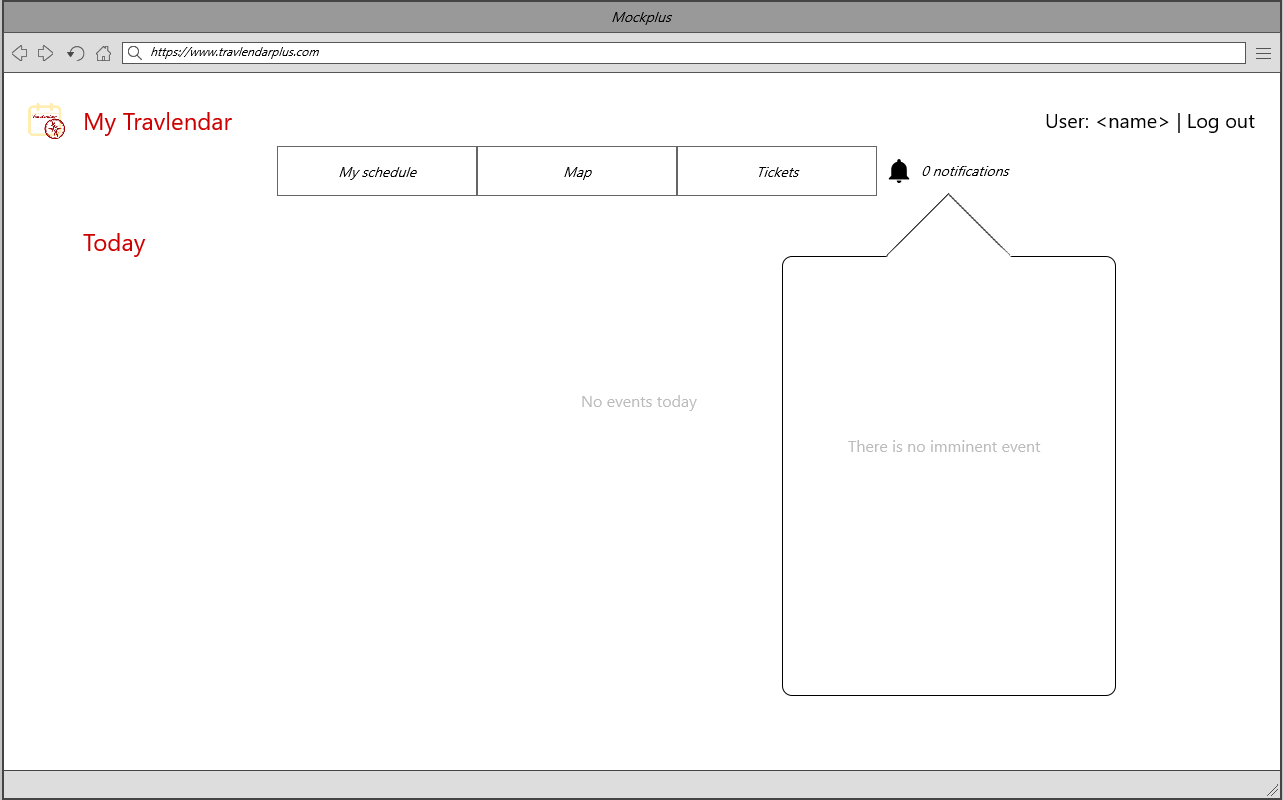
\includegraphics[width=\linewidth]{Images/Mockup/Web/07-web_homepage.png}
			\caption{\textbf{Web:} Home Page and Notifications}
			\label{fig:MU7}
			\end{figure}
			\begin{figure}[H]
			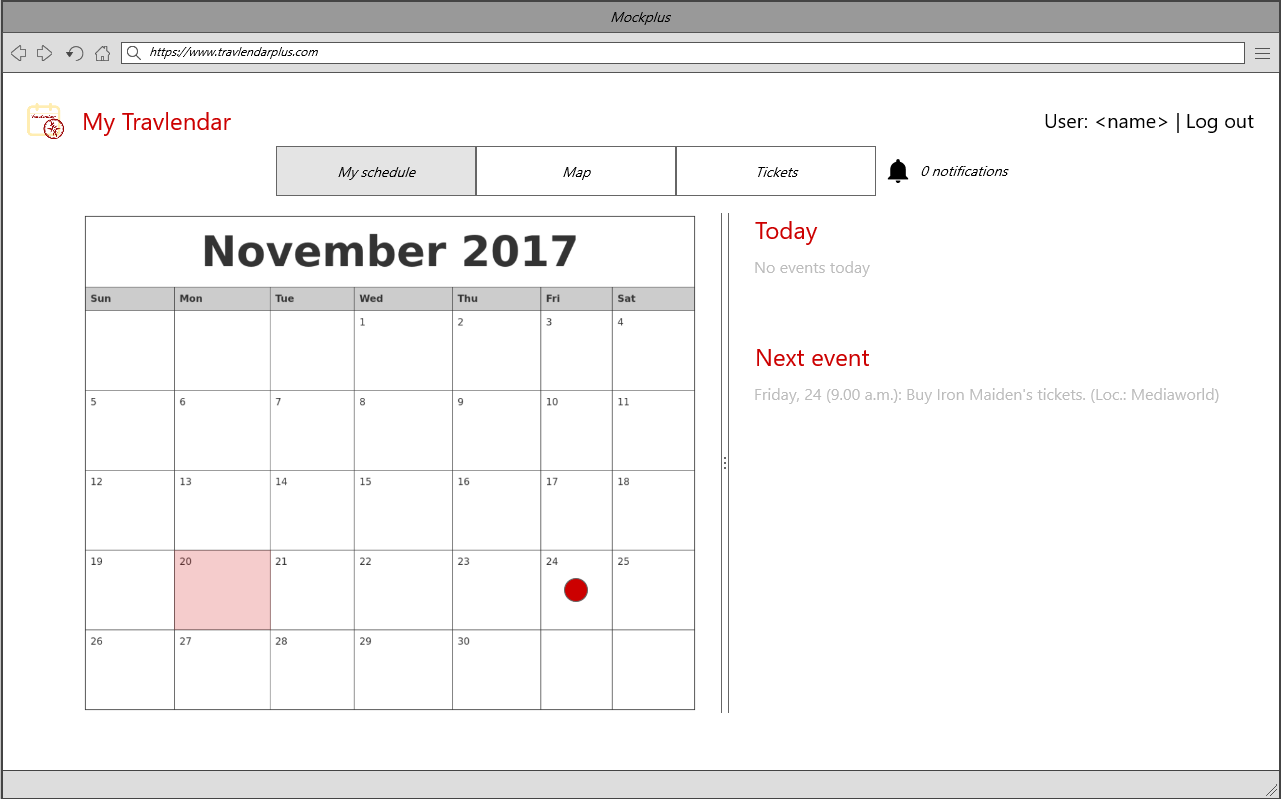
\includegraphics[width=\linewidth]{Images/Mockup/Web/08-web_Schedule.png}
			\caption{\textbf{Web:} Schedule}
			\label{fig:MU8}
			\end{figure}
			\begin{figure}[H]
			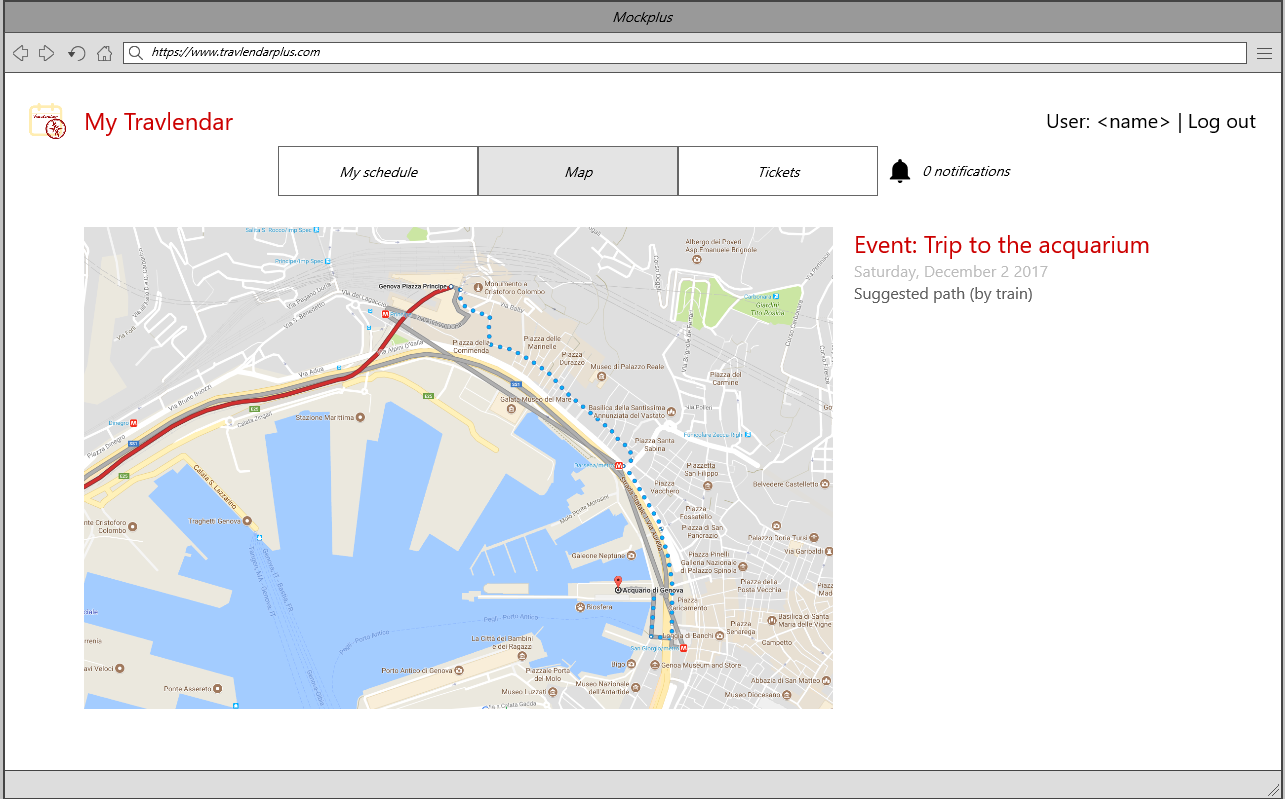
\includegraphics[width=\linewidth]{Images/Mockup/Web/09-web_Map.png}
			\caption{\textbf{Web:} Map showing a suggested path}
			\label{fig:MU9}
			\end{figure}
			\begin{figure}[H]
			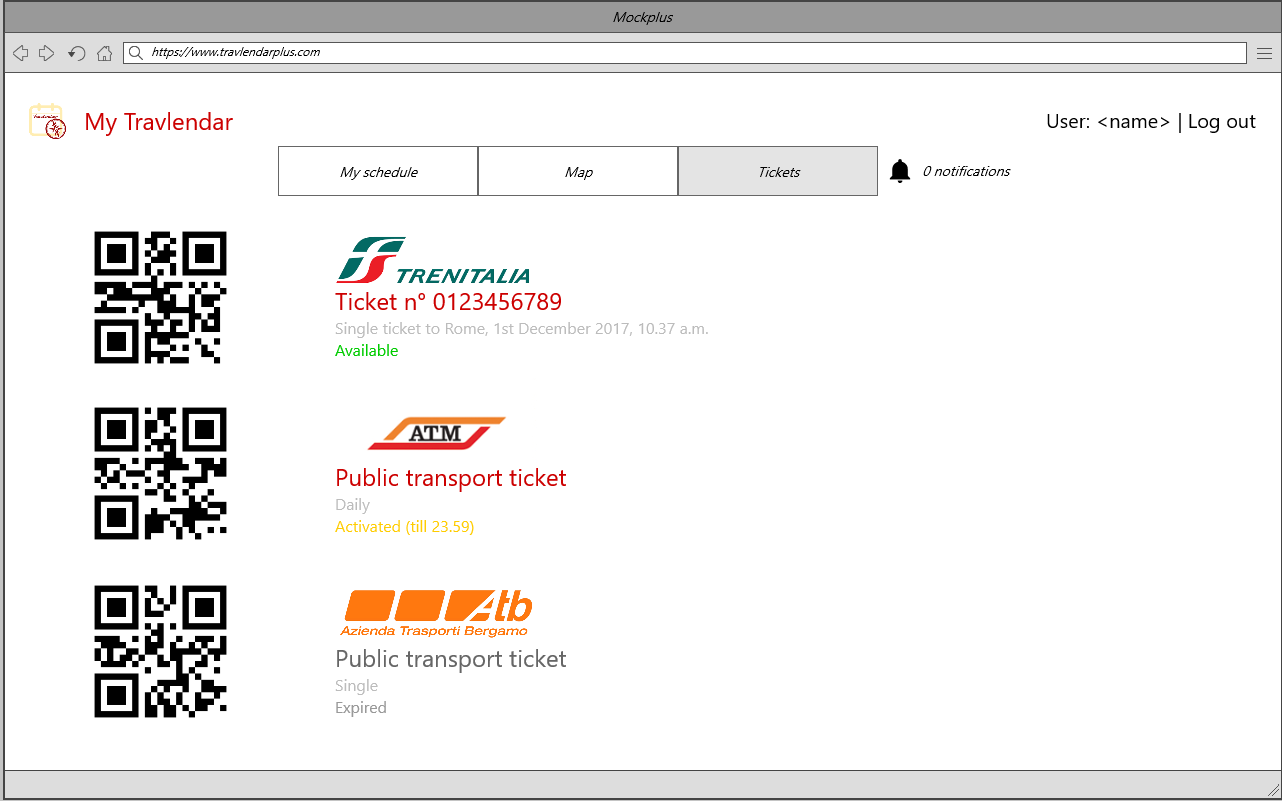
\includegraphics[width=\linewidth]{Images/Mockup/Web/10-web_Tickets.png}
			\caption{\textbf{Web:} Tickets}
			\label{fig:MU10}
			\end{figure}
		\subsection{UX Diagram}
			\paragraph{}The UX diagram provides deep informations about the interaction both with the mobile app and the web app. It is based on the class diagram graphical principles and features 3 kinds of objects: $<$$<$screen$>$$>$ for main pages, $<$$<$screen compartment$>$$>$ for page’s elements, and $<$$<$input form$>$$>$ for pages with the purpose to enter user’s data.
			\begin{figure}[H]
			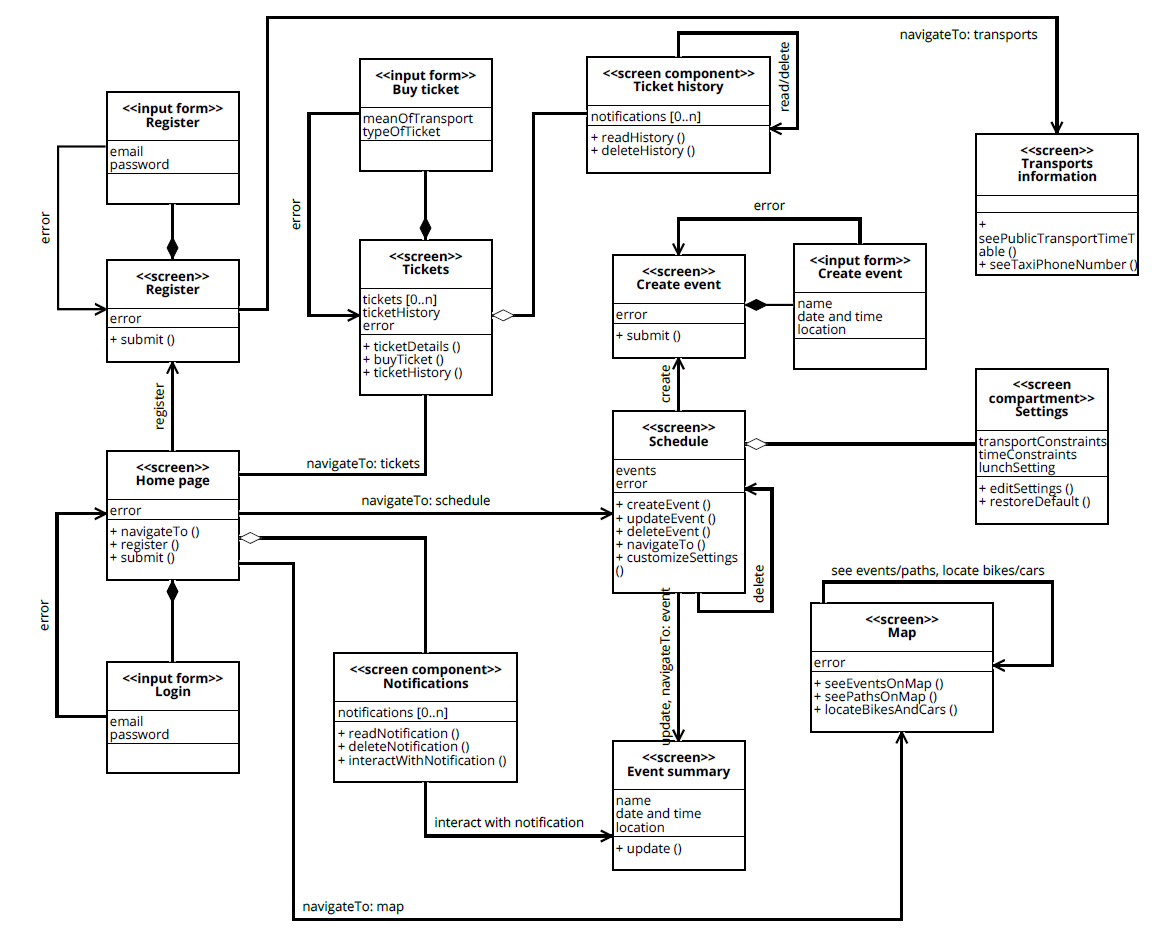
\includegraphics[width=\linewidth]{Images/Mockup/UX_BCE/UX.png}
			\caption{}
			\label{UX}
			\end{figure}
		\newpage
		\subsection{BCE Diagram}
			\paragraph{}The BCE diagram coniugate the UX diagram with the MVC pattern. The elements of the UX, which belong to the “View” are linked to the corresponding “Control” objects which operate on the Entities (the “Model”, according to MVC).
			\begin{figure}[H]
			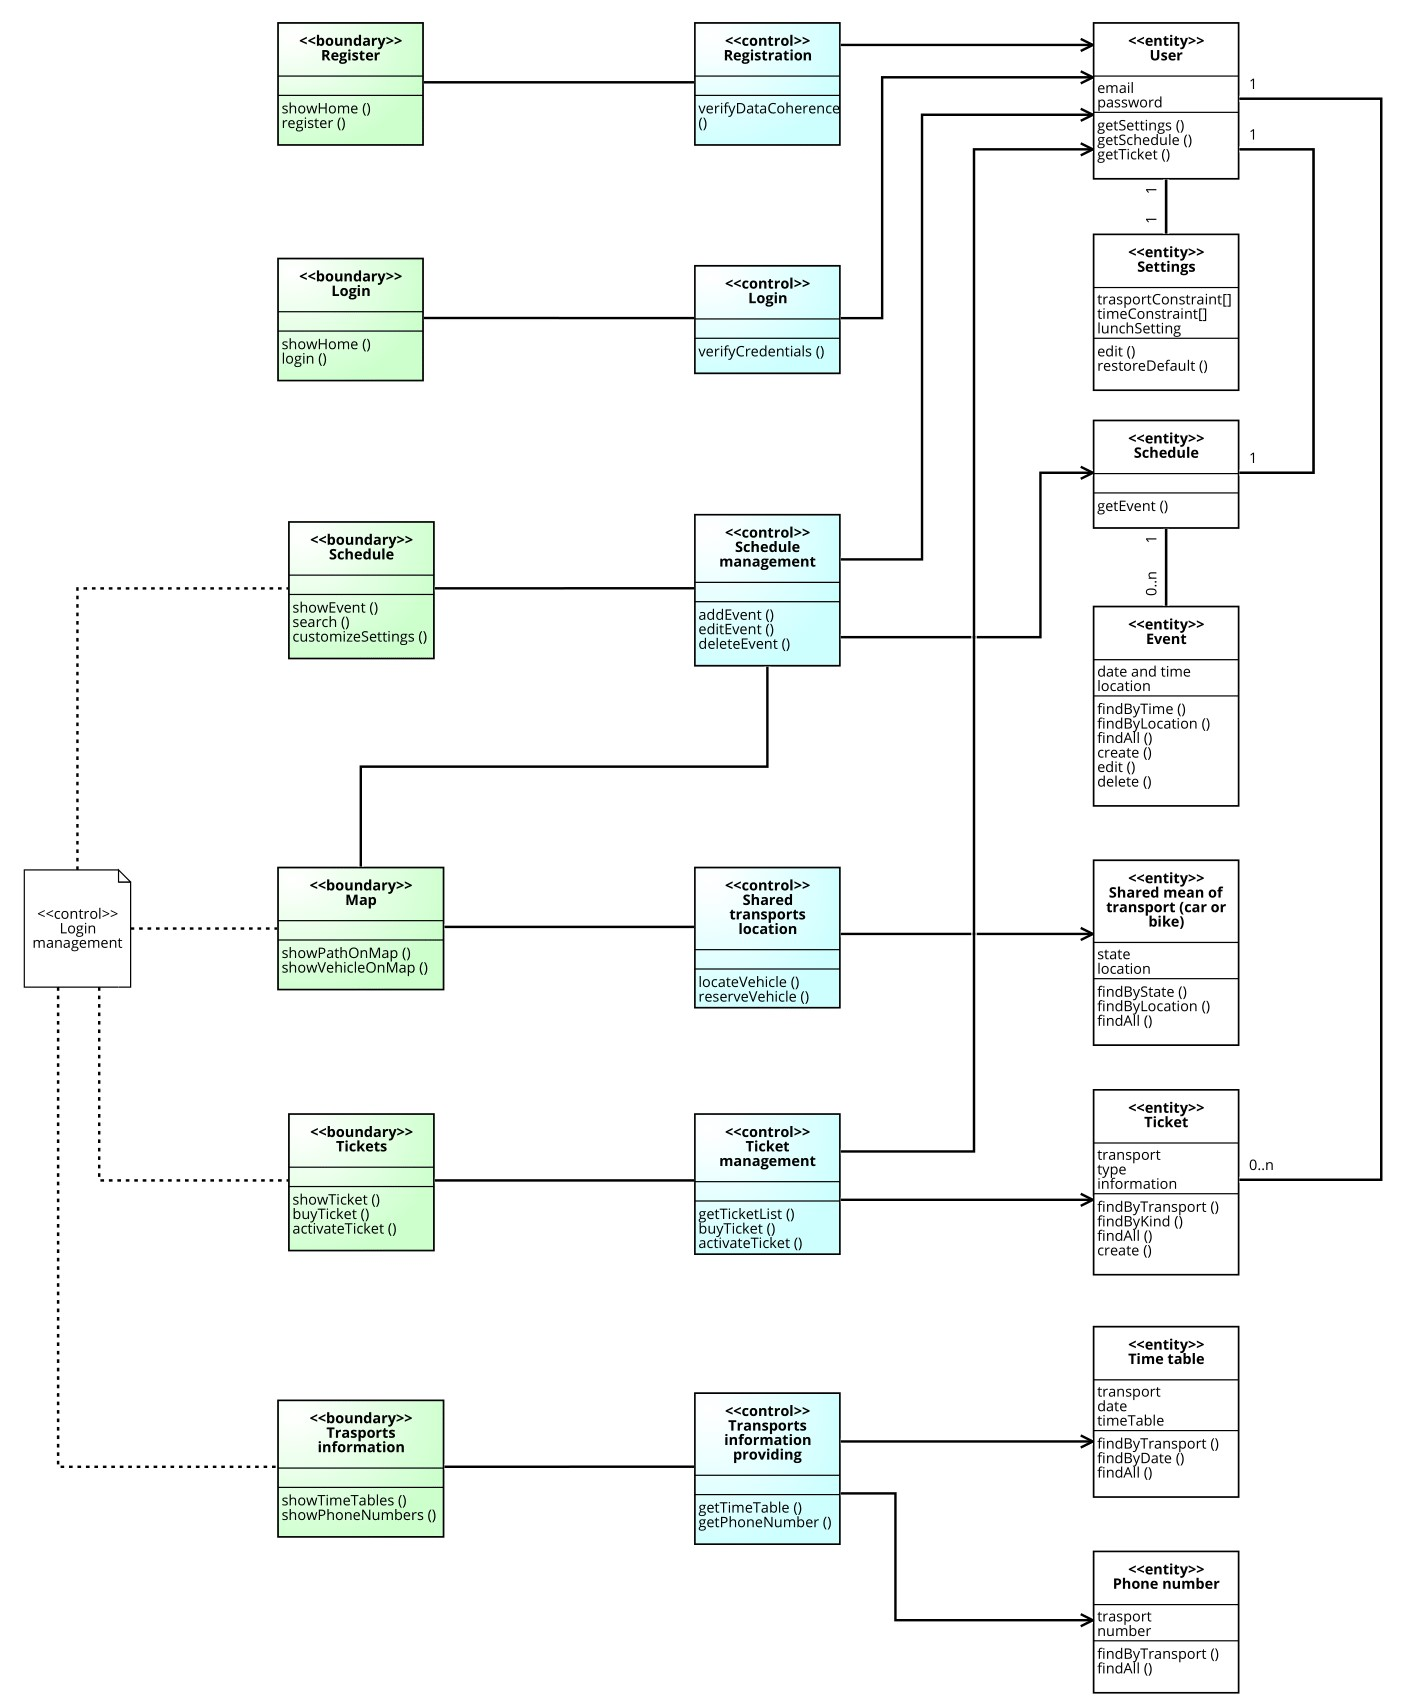
\includegraphics[width=\linewidth]{Images/Mockup/UX_BCE/BCE.jpg}
			\caption{}
			\label{BCE}
			\end{figure}			
	\section{Requirements Traceability}
		\paragraph{}In this section of the Design Document we will analyze the relationship between the components defined above in the document and the goals and requirements that were described in the RASD.
		\paragraph{Goal G1:}Allow a guest user to register to Travlendar+ by filling the registration form with the data needed.
		\begin{itemize}
		\item{}User Application Service: Account Manager.
		\item{}Requirements from R1 to R4.
		\end{itemize}
		\paragraph{Goal G2:}Allow the user to select preferences and modify them whenever he wants.
		\begin{itemize}
		\item{}User Application Service: Account Manager.
		\item{}Requirements from R5 to R7.
		\end{itemize}
		\paragraph{Goal G3:}Allow the user to easily create an organized and customizable agenda based on his preferences.
		\begin{itemize}
		\item{}User Application Service: Account Manager, Event Module, Schedule Module.
		\item{}Requirements R8 and R9.
		\end{itemize}
		\paragraph{Goal G4:}To help the user plan his movements in a clever and efficient way.
		\begin{itemize}
		\item{}User Application Service: Account Manager, Schedule Module, Ticket Module, Vehicle Module.
		\item{}Requirements from R10 to R13.
		\end{itemize}
		\paragraph{Goal G5:}To guarantee the user no to be late for his appointments.
		\begin{itemize}
		\item{}User Application Service: Schedule Module, Ticket Module, Vehicle Module.
		\item{}Requirements R14 and R15.
		\end{itemize}
		\paragraph{Goal G6:}To let the user buy bus or train tickets (both single and seasonal).
		\begin{itemize}
		\item{}User Application Service: Ticket Module.
		\item{}Requirements from R16 to R20.
		\end{itemize}
		\paragraph{Goal G7:}To let the user find vehicles from vehicle sharing systems.
		\begin{itemize}
		\item{} User Application Service: Vehicle Module.
		\item{} Requirement R21.
		\end{itemize}
		\paragraph{Goal G8:}Allow the user to buy in advance tickets which can be used later on.
		\begin{itemize}
		\item{} User Application: Account Manager, Ticket Module.
		\item{} Requirements from R22 to R25.
		\end{itemize}
	\newpage
	\section{Implementation, Integration and Test Plan}
		\subsection{Requirements and Entries}
		\paragraph{}External APIs should be available to guarantee a correct interaction with the navigation service, transport services, ticket dealers and payment gateway.\\Most of the components rely on DBMS. This means that the DBSM should be integrated and tested first.\\Some components relying on DBMS refer to a specific user, so the Account Manager should be integrated before them.\\The Schedule Manager should be integrated after the Event Manager, to be able to test it with concrete data.
		\subsection{Elements to be integrated and dependencies}
		\paragraph{}The software components are all enclosed in the User Application Service, the only subsystem. Most of them are independent one from each other, except for the Account Manager which is required by many other components and the Event Manager required by the Schedule Manager.\\The components and their dependencies are:
		\begin{itemize}
		\item{}Account Manager
			\begin{itemize}
			\item{}DBMS
			\end{itemize}
		\item{} Event Module
			\begin{itemize}
			\item{}DBMS
			\item{}Google Maps API
			\item{}Account Manager
			\end{itemize}
		\item{} Ticket Module
			\begin{itemize}
			\item{}DBMS
			\item{}Payment Gateway
			\item{}Public Transportation Services API
			\item{}Account Manager
			\end{itemize}
		\item{}Schedule
			\begin{itemize}
			\item{}DBMS
			\item{}Google Maps API
			\item{}Account Manager
			\item{}Schedule Module
			\end{itemize}
		\item{}Vehicle
			\begin{itemize}
			\item{}Google Maps API
			\item{}Vehicle Services API
			\end{itemize}
		\end{itemize}
		\subsection{Integration Strategy}
		\paragraph{}Having verified that the external APIs and the DBMS are working, the first components to be integrated should be the Account Manager and the Event Manager, to allow other components to work properly. The remaining components can be integrated in any order, allowing their development to be parallelized. The most suitable testing to start with  is bottom-up, so it is possible to check units and subcomponents up to the main component, User Application Service. Critical modules (we consider all subcomponents described in section Components View) integration testing will follow. Server-side of the application has highest priority in our development schedule (see Gantt Diagram provided below in this section).
			\begin{figure}[H]
			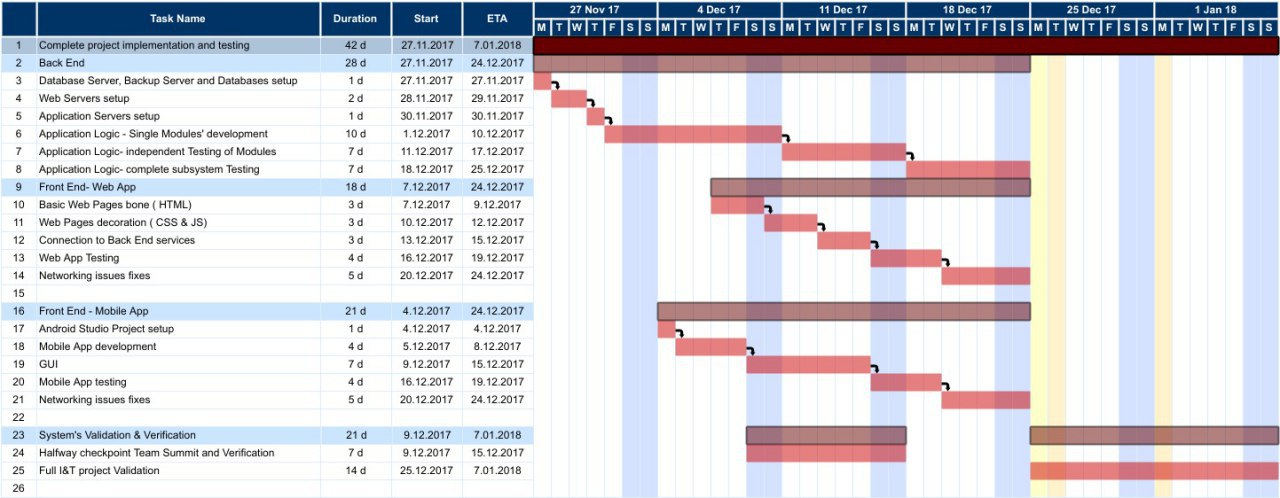
\includegraphics[width=\linewidth]{Images/Gantt_Diagram.jpg}
			\caption{Gantt Diagram}
			\label{Gantt}
			\end{figure}
		\newpage
		\subsection{Tools And Test Equiment}
			\subsubsection{Used Tools for Testing}
			\begin{itemize}
			\item{}\href{http://junit.org/junit5/}{Junit}
			\item{}\href{http://site.mockito.org/}{Mockito}
			\item{}\href{http://arquillian.org/}{Arquillian}
			\item{}\href{http://jmeter.apache.org/}{JMeter}
			\end{itemize}
			\subsubsection{Equipment}
			\paragraph{Front-end}
			\begin{itemize}
			\item{}\textbf{Mobile Application:} the mobile app will be developed for the mobile OS Android using the IDE Android Studio and its integrated simulator.
			\item{}\textbf{Web Application:} the web application will be tested on several browsers, OS and resolutions.
			\end{itemize}
			\paragraph{Back-end}
			\begin{itemize}
			\item{}\textbf{Application Server:} the server application will be developed using Java EE with the IDE NetBeans.
			\item{}\textbf{Web Server:}  it will be used an Apache HTTP server.
			\end{itemize}
	\newpage
	\section{Effort Spent}
		\begin{itemize}
		\item{Fumagalli Paolo:} $\sim$ 30 hours.
		\item{Grotti Pietro:} $\sim$ 30 hours.
		\item{Gullo Marco:} $\sim$ 30 hours.
		\end{itemize}
	\section{References}
		\begin{itemize}
		\item{} Google Doc
		\item{} Signavio
		\item{} Alloy Analyzer 4.2
		\item{} StarUML 5.3
		\item{} TeXworks
		
		\end{itemize}
\end{document}
